% !TeX program = pdflatex
% Overleaf: upload the complete RES-AI-Overleaf.zip project; main document main.tex.
% Local build: pdflatex main; bibtex main; pdflatex main; pdflatex main.
% Tables are inline; references are maintained in bibliography.bib.
% Empirical claims distinguish completed studies and the ChatDev subset from the unfinished cross-artifact campaign.
\documentclass[pdflatex,sn-mathphys-num]{sn-jnl}
\usepackage[T1]{fontenc}
\usepackage{lmodern}
\usepackage[english]{babel}
\usepackage{graphicx,booktabs,tabularx,multirow}
\newcolumntype{Y}{>{\raggedright\arraybackslash}X}
\usepackage{amsmath,amssymb,amsfonts,amsthm}
\usepackage{algorithm,algorithmicx}
\usepackage[noend]{algpseudocode}
\usepackage[expansion=false]{microtype}
\usepackage{tikz}
\usetikzlibrary{arrows.meta,positioning,fit,calc}
\usepackage{tcolorbox}
\tcbset{rqbox/.style={colback=gray!5, colframe=black!65, colbacktitle=gray!18, coltitle=black,
  fonttitle=\bfseries\small, fontupper=\small, boxrule=0.5pt, arc=1pt, left=5pt, right=5pt,
  top=3pt, bottom=3pt, toptitle=2pt, bottomtitle=2pt, before skip=8pt, after skip=8pt}}
\usepackage{url,placeins,hyperref}
\hypersetup{colorlinks=true,linkcolor=black,urlcolor=black,citecolor=black,hypertexnames=false}
% The Springer bibliography style's default \burl uses \textsf; URLs need \url
% so DOI underscores and other URL characters remain valid TeX.
\providecommand{\burl}[1]{}
\renewcommand{\burl}[1]{\url{#1}}
\theoremstyle{thmstylethree}
\newtheorem{definition}{Definition}
\newcommand{\tool}{\textsc{RES-AI}}
\newcommand{\upstream}{\texttt{use-hpc}}
\newcommand{\code}[1]{\texttt{#1}}

% BEGIN inline: generated/counts.tex
\newcommand{\LocalDecisions}{1040}
\newcommand{\LocalSeeds}{20}
\newcommand{\FaultFamilies}{12}
\newcommand{\CasesPerCondition}{260}
\newcommand{\MutationFaultCases}{240}
\newcommand{\MutationCleanCases}{20}
\newcommand{\StaticBlocked}{40}
\newcommand{\SmokeAdditional}{20}
\newcommand{\AblationVariants}{5}
\newcommand{\SensitivityAssessments}{9180}
\newcommand{\SensitivitySettings}{12}
\newcommand{\RefinementEpisodes}{1400}
\newcommand{\RefinementProposals}{1024}
\newcommand{\RefinementScienceChanged}{0}
\newcommand{\HeadroomGapSeeds}{6}
\newcommand{\OverheadRepeats}{200}
\newcommand{\OverheadMinAttempts}{2}
\newcommand{\OverheadMaxAttempts}{2048}
\newcommand{\OverheadMinMs}{0.022}
\newcommand{\OverheadMaxMs}{6.0}
\newcommand{\AnalysisPython}{3.13.14}

% END inline: generated/counts.tex

\raggedbottom
\setlength{\textfloatsep}{12pt plus 2pt minus 4pt}
\begin{document}
\title[RES-AI: Evidence-Bound Readiness for Shared HPC]{RES-AI: Evidence-Bound Readiness for AI Software Engineering Experiments on Shared HPC Infrastructure}
\author*[1]{\fnm{Majid} \sur{Babaei}}\email{majid.babaei@ufv.ca}
\affil*[1]{\orgdiv{School of Computing}, \orgname{University of the Fraser Valley}, \orgaddress{\state{BC}, \country{Canada}}}
\abstract{Researchers across software engineering increasingly conduct experiments in or for AI systems. Executing them on shared clusters introduces a gap between a successful small test and justified admission of a larger job. Configuration checks alone cannot establish that evidence still describes the submitted workload, that required probes ran, or that a successful process produced valid outputs. We present RES-AI, a research prototype separating the scientific specification from its execution plan and evaluating a bounded readiness contract before production submission. The contract binds evidence to the current plan, requires coverage, freshness, memory headroom and repeated observations, and charges failed attempts against the validation budget. A restricted Model Context Protocol interface exposes assessment and refinement proposals to agents; existing Slurm templates provide execution and auditing. An executed synthetic mutation study comprises \LocalDecisions{} policy decisions over \FaultFamilies{} fault families and clean controls. The full policy blocks all \MutationFaultCases{} faulty variants and accepts all \MutationCleanCases{} clean variants in this deliberately constructed suite, whereas a static validator blocks \StaticBlocked{} and a smoke proxy 60. A leave-one-conjunct-out ablation shows that each of the five contract components detects faults no other check detects. Threshold sweeps, \RefinementEpisodes{} simulated refinement episodes and latency measurements show that decisions follow declared parameters, that charged validation stays within its cap without altering the scientific specification, and that assessment costs milliseconds. They also expose two specification gaps. These results establish implementation behavior under specified inputs, not field failure rates or resource savings. A bounded MapCoder deployment case study additionally executes two fresh repeats under each of two local models, Qwen2.5-Coder-7B and quantized Qwen3.8-27B; all four executions solve one HumanEval task and pass their declared probes, without establishing aggregate accuracy or comparative savings. A real-GPU integration pilot and a completed 140-episode ChatDev comparison extend this evidence. Across five paired task/seed blocks, the full policy blocks all 15 injected-fault cases and completes all five clean cases; smoke-then-production blocks 10 of 15 faults. Three historical attempts with ineffective fault injection are quarantined and excluded. These descriptive single-artifact results do not establish cross-artifact effects. Eleven of twelve planned artifact comparisons remain unstarted; production-scale reliability and compute savings remain unestablished.}
\keywords{empirical software engineering, AI agents, shared HPC, Slurm, experimental validation, reproducibility, Model Context Protocol}
\maketitle

\section{Introduction}\label{sec:introduction}
An increasing share of software engineering researchers are becoming researchers in or for AI systems. The speed of AI development and its growing role in software construction make experimental execution part of the research method itself. Evaluations of code generation, repository repair and software development agents execute generated programs, construct environments, and interact with models over many tasks and seeds. SWE-bench and SWE-agent illustrate this move toward repository-level execution, while rigorous code-generation evaluation requires more than superficial output checks \cite{jimenez2024swebench,yang2024sweagent,liu2023evalplus}. Scientific conclusions therefore depend on both the approach under investigation and the infrastructure that actually runs it.

Shared high-performance computing (HPC) makes substantial experiments accessible without requiring each research group to own an accelerator fleet. It introduces constraints absent from a workstation: allocations expire, resources are heterogeneous, software stacks differ across nodes, and admission follows site policy. A malformed configuration can fail quickly; an input-dependent memory fault or broken checkpoint can remain hidden much longer. A process can also exit successfully while writing incomplete data. Repeated submission without a clear validation contract consumes resources and delays both the researcher and other cluster users.

Reproducibility initiatives emphasize executable artifacts and explicit experimental context \cite{pineau2021improving,acm2020badges}. For reviewers, a practical question is whether a result can be regenerated from declared inputs. For an organization considering adoption, it is whether the artifact operates within its resource and deployment constraints. Neither question is answered by a successful scheduler exit code alone. Scientific benchmarking also requires clear measurement conditions and treatment of variation \cite{hoefler2015scientific}. Resource use matters because validation itself has a cost: a preflight consuming more compute than it saves is not automatically beneficial.

Three gaps motivate this work. First, static validity and execution validity differ: a valid job graph can fail to initialize a model or satisfy an output contract. Second, evidence is conditional: a successful smoke run can become irrelevant after a model, input, software or resource change. Third, validation coverage and cost need to be represented together in the admission decision. An agent repeatedly modifying a workflow can amplify these gaps unless changes invalidate corresponding evidence and retries remain bounded.

We address these gaps with \tool{}, an evidence-bound readiness layer above a Slurm execution engine. A scientific specification identifies the intended experiment; an execution plan identifies how it runs. Smoke probes produce observations against declared obligations. The readiness gate accepts only fresh, matching, sufficiently complete evidence within a budget. A permitted refinement creates a new plan identity and requires new evidence. A small Model Context Protocol (MCP) interface lets agents inspect eligibility without unrestricted submission privileges.

The contribution is narrower than a new scheduler or a reproducibility guarantee. We reuse the job-graph, runner and audit templates supplied by \upstream{} and identify their pinned revision. We do not claim priority escalation: a short, accurate time request can improve backfill eligibility, but the scheduler controls admission \cite{schedmdScheduling}. A small probe also cannot establish that a many-node, multi-day experiment will succeed.

We make four contributions: (1) a readiness contract over scientific identity, execution identity, coverage, resource observations and validation cost; (2) a Python prototype with conservative assessment, bounded refinement proposals, an operator-facing submission wrapper and restricted MCP tools; (3) executed controller studies (a mutation study, a component ablation, a threshold sensitivity analysis, a bounded-refinement simulation and an overhead measurement), a Slurm GPU integration pilot, and a one-artifact deployment case study with two local-model configurations, all regenerated from archived records; and (4) a twelve-artifact evaluation protocol with a completed, audited 140-episode ChatDev subset separating infrastructure reliability, scientific preservation and total resource cost. This subset provides descriptive evidence for one artifact; the cross-artifact analysis remains incomplete.

\section{Background and Running Example}\label{sec:background}
\subsection{Shared resources and empirical AI studies}
Slurm manages resource requests, allocation and execution \cite{yoo2003slurm}. A partition defines an administrative resource set and its constraints; accounts and quality-of-service policies determine what a user may request. Dependencies express job precedence, and arrays represent repeated experiment cells. Backfill can start a lower-priority request when doing so does not delay a higher-priority job's expected start. It depends on requested resources and time limits rather than an application independently acquiring priority \cite{schedmdScheduling}.

For an AI experiment, allocation is only one part of the context. Weights, tokenizer, data revision, input lengths, precision, prompts, test harness and seeds can affect both demand and outcomes. Serving systems such as vLLM explicitly manage inference memory \cite{kwon2023vllm}; an orchestration layer should not infer numerical reproducibility from available memory. A valid deployment is a prerequisite for evaluating an approach, not evidence of its effectiveness.

Workflow systems already automate dependencies and execution across resources \cite{deelman2015pegasus,molder2021snakemake,babuji2019parsl}, containers improve portability \cite{kurtzer2017singularity}, and context capture supports computational reuse \cite{davison2012sumatra,crusoe2022cwl}. Our question is consequently not whether jobs can be orchestrated, but when validation evidence justifies dispatch of a particular production specification.

\subsection{An illustrative running example}
Consider a team evaluating a multi-agent code-generation framework across 64 GPUs. Its pipeline loads models, distributes tasks, executes generated programs and aggregates results. A long input could exceed memory, a worker could fail to join a collective, or aggregation could drop unfinished tasks. A fault appearing on the third day would be expensive, but the day and scale in this example are hypothetical, not measurements from our study.

A short single-GPU test exercises imports and loading, but not necessarily maximum input size, checkpoint recovery or inter-node communication. It provides evidence for its exercised obligations, not readiness for the complete 64-GPU plan. \tool{} makes the missing obligations explicit. The team must add representative boundary-input, checkpoint and distributed probes, or narrow its claim. No fixed fifteen-minute turnaround is promised: the queue and required test scale determine the actual time.

Suppose a boundary-input probe approaches the memory limit. Reducing an inference microbatch can be operational if the experiment permits it and preserves intended outcomes. Reducing effective training batch size can change the experiment. The implemented proposal therefore requires a scientific declaration of batch invariance, which must separately be tested. An out-of-memory event never authorizes changing the model, data or evaluation metric.

\subsection{Identity, topology and evidence}
Definitions are needed because a pass/fail flag without scope is ambiguous. We first distinguish intended science from execution configuration, then identify the evidence connecting them.
\begin{definition}[Experiment identity]
Let $S$ be the scientific specification, $X$ the execution plan, $O$ the mandatory probe set, $B$ the validation policy and budget, and $I$ declared input identities. The plan identity is $h=H(S,X,O,B,I)$, using canonical SHA-256. $S$ records scientific choices such as model, data, prompts, seeds and scoring; $X$ records resource shape and operational settings; $I$ binds declared files to full content hashes.
\end{definition}
Changing $X$ invalidates old-plan evidence; changing $S$ additionally changes the scientific experiment. Hash equality establishes identity of declared content, not authenticity, exhaustive dependency capture or deterministic execution.

Topology can inform feasible request shapes and probe selection, but scheduler descriptions need not measure physical network performance. Unknown attributes must remain explicit.
\begin{definition}[Observed resource graph]
A resource snapshot is $G_t=(V_t,E_t,A_t)$, with timestamp $t$, advertised nodes or accelerators $V_t$, topology relations $E_t$ and attributes $A_t$. Edge bandwidth and latency may be unknown. Scheduler-reported relations and measurements inside allocations are distinct evidence sources.
\end{definition}
Discovery archives what the scheduler reports; it neither reconstructs measured link weights nor optimizes placement. In the example, sharing an advertised switch does not replace a distributed probe at the required allocation shape.

Each attempt must identify what it exercised and observed. Otherwise successful execution can be mistaken for comprehensive validation.
\begin{definition}[Smoke evidence]
An attempt record $e_i$ contains a distinct identifier, plan hash $h_i$, timestamp $t_i$, process status, passed obligations $C_i$, output validity, peak memory fraction $m_i$ and allocated-instance process time $c_i$. Bundle $E$ retains all supplied attempts, including failed and obsolete attempts.
\end{definition}
Obligations can include imports, model initialization, a boundary input, output schema/count, checkpoint round trip and distributed collective completion. Their implementation is workload-specific; names alone do not establish adequate testing. The CUDA pilot implements the first five for a small synthetic network and contains no distributed probe.

Readiness is a conjunction so an obligatory failure cannot be hidden by an average score. With the two most recent matching attempts $e_a,e_b$, lifetime $T$, memory limit $m_{\max}$, stability tolerance $\epsilon$, attempt cap $K$ and compute cap $C$, the rule is
\begin{align}
\operatorname{Ready}(P,E,t)={}&\operatorname{Valid}(P)\land |E|\leq K\land\sum_{e_i\in E}c_i\leq C \label{eq:ready}\\
&\land\bigwedge_{i\in\{a,b\}}[h_i=h\land\operatorname{OK}(e_i)\land O\subseteq C_i\land\operatorname{OutputValid}(e_i)]\nonumber\\
&\land\bigwedge_{i\in\{a,b\}}[0\leq t-t_i\leq T\land0\leq m_i\leq m_{\max}]\land\Delta_{\mathrm{smoke}}\leq\epsilon,\nonumber
\end{align}
where $P=(S,X,O,B,I)$ and $\Delta_{\mathrm{smoke}}=|m_a-m_b|$. Records are ordered by timestamp for selection. All attempt identifiers must be nonempty and unique; every $c_i$ must be positive and finite. Missing evidence blocks readiness. Distinct executions do not establish statistical independence. Memory difference is a stability diagnostic, not a convergence theorem for stochastic agents.


% BEGIN inline: sections/approach.tex
\section{Approach}\label{sec:approach}
\subsection{Overview}\label{sec:approach-overview}
Figure~\ref{fig:approach-overview} organizes \tool{} into three tiers. An access tier separates an AI agent, which reaches the system only through restricted MCP tools, from the operator, who executes probes, reviews proposals and requests dispatch. The middle tier is the \tool{} readiness layer, whose six numbered components connect an experiment plan to an admission decision. The bottom tier is the inherited execution substrate: the pinned \upstream{} templates and the Slurm scheduler of the shared cluster. \tool{} adds the readiness layer and reuses the substrate unchanged.

\begin{figure}[t]
\centering

% BEGIN inline: figures/approach_overview.tex
% RES-AI architecture overview (Figure fig:approach-overview); requires tikz.
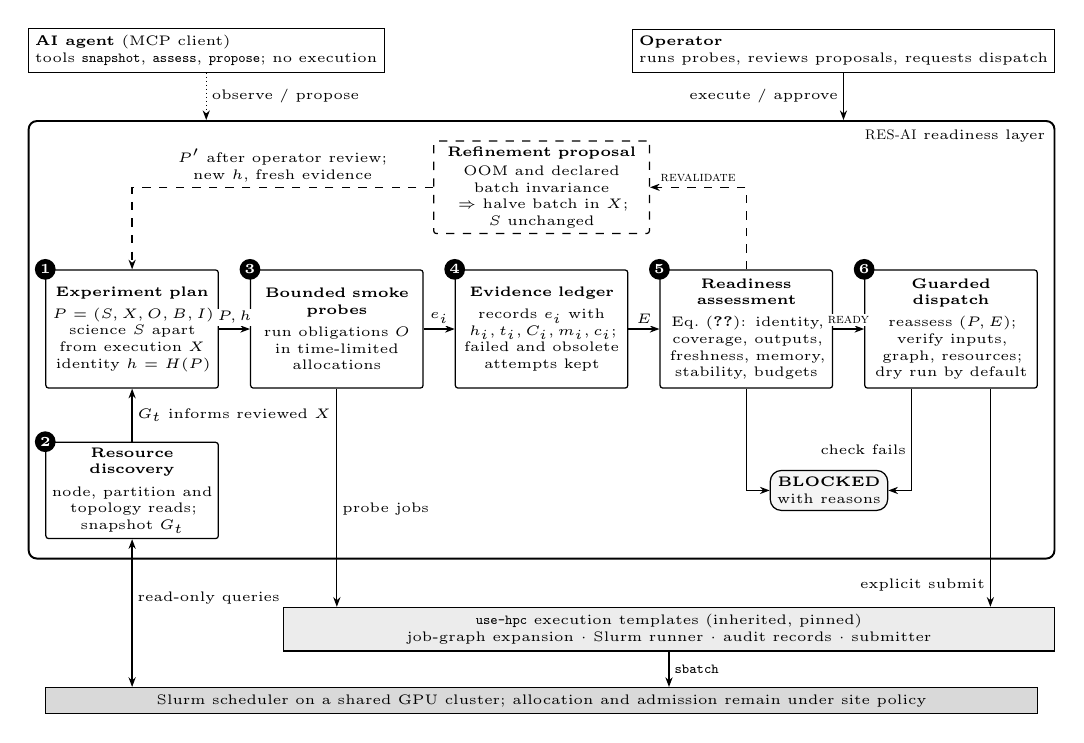
\begin{tikzpicture}[
  font=\tiny, >={Stealth[length=3.5pt,width=2.6pt]}, line width=0.45pt,
  comp/.style={draw, rounded corners=1pt, fill=white, text width=2.05cm,
    minimum height=1.5cm, align=center, inner sep=2pt},
  num/.style={circle, fill=black, text=white, inner sep=0pt, minimum size=7.5pt,
    font=\tiny\bfseries},
  term/.style={draw, rounded corners=4pt, fill=gray!8, align=center, inner sep=2.5pt},
  inherited/.style={draw, fill=gray!15, align=center, inner sep=2.5pt},
  actor/.style={draw, fill=white, align=left, inner sep=2.5pt},
  flow/.style={->},
  rev/.style={->, dashed},
  lbl/.style={fill=white, inner sep=0.8pt},
]
% Readiness layer: (1) plan -> (3) probes -> (4) ledger -> (5) assessment -> (6) dispatch.
\node[comp] (plan) at (1.05,0) {\textbf{Experiment plan}\\[2pt]
  $P=(S,X,O,B,I)$\\ science $S$ apart\\ from execution $X$\\ identity $h=H(P)$};
\node[comp] (smoke) at (3.65,0) {\textbf{Bounded smoke}\\ \textbf{probes}\\[2pt]
  run obligations $O$\\ in time-limited\\ allocations};
\node[comp] (ledger) at (6.25,0) {\textbf{Evidence ledger}\\[2pt]
  records $e_i$ with\\ $h_i,t_i,C_i,m_i,c_i$;\\ failed and obsolete\\ attempts kept};
\node[comp] (assess) at (8.85,0) {\textbf{Readiness}\\ \textbf{assessment}\\[2pt]
  Eq.~(\ref{eq:ready}): identity,\\ coverage, outputs,\\ freshness, memory,\\ stability, budgets};
\node[comp] (dispatch) at (11.45,0) {\textbf{Guarded dispatch}\\[2pt]
  reassess $(P,E)$;\\ verify inputs,\\ graph, resources;\\ dry run by default};
\node[comp, minimum height=1.0cm] (discover) at (1.05,-2.05) {\textbf{Resource}\\ \textbf{discovery}\\[2pt]
  node, partition and\\ topology reads;\\ snapshot $G_t$};
\node[comp, dashed, minimum height=0.8cm, text width=2.6cm] (refine) at (6.25,1.8)
  {\textbf{Refinement proposal}\\[1pt] OOM and declared\\ batch invariance\\ $\Rightarrow$ halve batch in $X$;\\ $S$ unchanged};
\node[term] (blocked) at (9.9,-2.05) {\textbf{BLOCKED}\\ with reasons};

\foreach \n/\k in {plan/1, discover/2, smoke/3, ledger/4, assess/5, dispatch/6}
  \node[num] at (\n.north west) {\k};

\draw[flow] (plan) -- node[lbl, above=1pt] {$P,h$} (smoke);
\draw[flow] (smoke) -- node[lbl, above=1pt] {$e_i$} (ledger);
\draw[flow] (ledger) -- node[lbl, above=1pt] {$E$} (assess);
\draw[flow] (assess) -- node[lbl, above=1pt] {\textsc{ready}} (dispatch);
\draw[flow] (discover) -- node[lbl, right=1pt] {$G_t$ informs reviewed $X$} (plan);
\draw[flow] (assess.south) |- (blocked.west);
\draw[flow] ([xshift=-0.5cm]dispatch.south) |- node[lbl, pos=0.3, left=1pt] {check fails} (blocked.east);
\draw[rev] (assess.north) |- node[lbl, pos=0.75, above=1pt] {\textsc{revalidate}} (refine.east);
\draw[rev] (refine.west) -| node[lbl, pos=0.25, above=1pt, align=center]
  {$P'$ after operator review;\\ new $h$, fresh evidence} (plan.north);

\node[fit=(plan)(dispatch)(discover)(blocked)(refine), draw, rounded corners=3pt,
  inner xsep=6pt, inner ysep=7pt, line width=0.7pt] (layer) {};
\node[anchor=north east, inner sep=3.5pt] at (layer.north east) {\tool{} readiness layer};

% Access tier: agents observe and propose; the operator executes and submits.
\node[actor, anchor=south west] (agent) at ([yshift=0.6cm]layer.north west)
  {\textbf{AI agent} (MCP client)\\ tools \code{snapshot}, \code{assess}, \code{propose}; no execution};
\node[actor, anchor=south east] (operator) at ([yshift=0.6cm]layer.north east)
  {\textbf{Operator}\\ runs probes, reviews proposals, requests dispatch};
\draw[->, densely dotted] (agent.south) -- node[lbl, right=1pt] {observe / propose}
  (agent.south |- layer.north);
\draw[->] (operator.south) -- node[lbl, left=1pt] {execute / approve}
  (operator.south |- layer.north);

% Inherited execution substrate.
\node[inherited, anchor=north east, minimum width=9.8cm] (usehpc)
  at ([yshift=-0.6cm]layer.south east)
  {\upstream{} execution templates (inherited, pinned)\\
   job-graph expansion $\cdot$ Slurm runner $\cdot$ audit records $\cdot$ submitter};
\node[inherited, fill=gray!30, anchor=north, minimum width=12.6cm] (slurm)
  at ([yshift=-0.45cm]layer.south |- usehpc.south)
  {Slurm scheduler on a shared GPU cluster; allocation and admission remain under site policy};
\draw[flow] (smoke.south) -- node[lbl, pos=0.55, right=1pt] {probe jobs} (smoke.south |- usehpc.north);
\draw[flow] ([xshift=0.5cm]dispatch.south) -- node[lbl, pos=0.9, left=1pt] {explicit submit}
  ([xshift=0.5cm]dispatch.south |- usehpc.north);
\draw[<->] (discover.south) -- node[lbl, pos=0.4, right=1pt] {read-only queries} (discover.south |- slurm.north);
\draw[flow] (usehpc.south) -- node[lbl, right=1pt] {\code{sbatch}} (usehpc.south |- slurm.north);
\end{tikzpicture}

% END inline: figures/approach_overview.tex

\caption{Layered architecture of \tool{}. Numbered components form the readiness layer; shaded tiers are inherited and unchanged. Solid arrows carry data or decisions: the plan $P$ and its identity $h$, attempt records $e_i$, accumulated evidence $E$ and the resource snapshot $G_t$. Dashed elements form the only revision path, which requires operator review, yields a new identity and invalidates earlier evidence for admission. The dotted agent connection permits observation and proposals but neither execution nor submission. OOM denotes out of memory.}\label{fig:approach-overview}
\end{figure}

The experiment plan (1) separates scientific choices $S$ from execution settings $X$ and records the mandatory probes $O$, validation policy $B$ and input identities $I$; its hash $h$ identifies the exact plan. Resource discovery (2) issues read-only scheduler queries and archives a snapshot $G_t$ that informs the reviewed choice of $X$. The scheduler retains control of allocation and admission.

Bounded smoke probes (3) exercise the declared obligations through the \upstream{} runner under explicit, time-limited allocations started by the operator. Each attempt yields a record $e_i$ in the evidence ledger (4), carrying its plan identity, timestamp, passed obligations, output validity, peak memory fraction and cost. Failed and obsolete attempts remain in the ledger for validation-cost accounting. Readiness assessment (5) evaluates Equation~\eqref{eq:ready} over the current plan and accumulated evidence $E$: identities must match, the two most recent observations must be fresh, complete, valid and stable, and attempt and compute budgets must hold. Missing or invalid evidence yields BLOCKED with reasons.

A READY decision passes to guarded dispatch (6), which reassesses readiness immediately before dispatch and verifies declared files, the resolved execution graph and the supported resource mapping. Any failed check yields BLOCKED. Otherwise the wrapper produces a dry run by default and invokes the upstream submitter only on explicit operator request.

The dashed path applies only when a permitted refinement exists. After a matching out-of-memory failure, assessment returns REVALIDATE with a proposal that halves the batch size in $X$, provided the scientific contract declares batch invariance; $S$ is never altered. The operator reviews the proposal and adopts the revised plan $P'$, whose new identity prevents reuse of earlier evidence, and collects fresh matching observations. Without an applicable proposal, the operator must diagnose the failure, obtain missing evidence or stop. Agents may call discovery, assessment and proposal tools, whereas probe execution and submission remain operator actions. Algorithms~\ref{alg:discover}--\ref{alg:dispatch} detail these interactions; unattended repair and resubmission are not implemented.

\begin{algorithm}[H]
\caption{DiscoverClusterTopology: archive resource observations}\label{alg:discover}
\begin{algorithmic}[1]
\Require Scheduler read interfaces
\Ensure Timestamped snapshot $G_t$ with explicit unknowns
\State $R\gets\emptyset$; $t\gets\Call{CurrentTime}{}$
\For{$q$ in \{node inventory, partitions, topology\}}
\State $R[q]\gets\Call{ReadWithTimeout}{q}$ \Comment{output, status or unavailable}
\EndFor
\State \Return $(R,t,\text{bandwidth unknown},\text{latency unknown})$
\end{algorithmic}
\end{algorithm}
\begin{algorithm}[H]
\caption{ExecuteSmokeTestLoop: assess a bounded iteration}\label{alg:smoke}
\begin{algorithmic}[1]
\Require Plan $P$, accumulated evidence $E$, snapshot $G_t$
\Ensure READY, REVALIDATE with proposal, or BLOCKED with reasons
\State \Call{CheckRequestFeasibility}{$P,G_t$} \Comment{operator checks site constraints}
\State $r\gets\Call{AssessReadiness}{P,E}$ \Comment{Equation~\ref{eq:ready}}
\If{$r.\mathrm{ready}$} \State \Return READY, $r$ \EndIf
\If{attempt or compute budget exhausted} \State \Return BLOCKED, $r$ \EndIf
\State $P'\gets\Call{ProposeRefinement}{P,E}$
\If{$P'\neq\bot$}
\State \Return REVALIDATE, $P'$ \Comment{collect new matching evidence}
\EndIf
\State \Return BLOCKED, $r$ \Comment{diagnose fault or obtain missing probes}
\end{algorithmic}
\end{algorithm}
\begin{algorithm}[H]
\caption{OrchestrateFullExperiment: operator-facing dispatch}\label{alg:dispatch}
\begin{algorithmic}[1]
\Require Plan $P$, evidence $E$, dispatch mode $d$ (dry-run by default)
\State $r\gets\Call{AssessReadiness}{P,E}$
\State $r.\mathrm{reasons}\gets r.\mathrm{reasons}\cup\Call{VerifyDeclaredInputs}{P}$
\State $r.\mathrm{reasons}\gets r.\mathrm{reasons}\cup\Call{ValidateExecutionGraph}{P}$
\State \Call{PrintDecision}{r}
\If{$r.\mathrm{reasons}\neq\emptyset$} \State \Return BLOCKED \EndIf
\State \Return \Call{UpstreamSubmit}{d} \Comment{explicit operator submission}
\end{algorithmic}
\end{algorithm}

\subsection{Resource discovery and request selection}
Algorithm~\ref{alg:discover} performs light metadata reads. Each read is bounded in time and preserves failures, preventing unavailable topology from silently becoming an apparently healthy empty cluster. Discovery archives what the operator can inspect; it does not place jobs.

Request selection respects authorized accounts, partitions, accelerator type, memory and walltime. Let $\mathcal{P}(j,t)$ denote the scheduler's priority for job $j$ at time $t$. It is observed or queried where available; it is not a value that \tool{} can independently increase. Selection resides in reviewed configuration. Short requests may create backfill opportunities, but their effect on waiting time must be measured. Discovery and monitoring must respect site limits on scheduler queries.

\subsection{Coverage-directed validation}
An obligation list explains why a probe is needed before execution. In the running example, imports and initialization test deployment, a boundary input tests a declared envelope, an output check tests schema/cardinality, a checkpoint probe tests recovery, and a collective probe tests communication. A test cannot satisfy an unexercised obligation by completing quickly. A single-GPU observation must not be relabeled as evidence for a distributed workload.

Algorithm~\ref{alg:smoke} uses the two most recent observations for the exact plan. Older or different-plan records do not establish readiness but retain their compute charges. A recent failed observation blocks admission even if an earlier attempt passed. Two observations reduce dependence on one accidental success; they do not characterize rare faults. Evidence expiry is a policy choice, not an empirically discovered boundary of resource stability.

The lifetime, memory envelope and validation budget are predeclared policy parameters rather than universal constants. Their experimental values appear in Section~\ref{sec:experimental-setup}. A production study must justify these choices for its workload and distinguish framework-allocated memory from all memory used on a device.

\subsection{Bounded refinement and scientific preservation}
A feedback mechanism needs permitted actions and stopping rules. The approach permits one action: halve a batch size greater than one after an out-of-memory classification, only if the scientific contract declares batch invariance and the failing evidence matches the plan. The action modifies the execution subdocument and never the scientific one, and it is returned as a proposal for operator review rather than executed.

The revised hash prevents old records from validating the new configuration. Two new matching observations are needed, with previous costs retained. Unknown faults produce no proposal. Attempt and compute caps bound assessment eligibility, and scheduler limits bound the actual allocation. An autonomous wall-clock budget controller is outside the scope of the approach.

Preserving JSON fields is necessary but insufficient for preserving the scientific estimand. Training batch changes can alter optimization; inference scheduling and numerical nondeterminism can alter outputs. The prospective campaign therefore tests permitted repairs against predeclared tolerances. A model substitution, precision change or revised dataset creates a new scientific specification rather than an invisible recovery action.

\subsection{Guarded execution and agent access}
The execution backend expands the experiment graph, submits dependencies, runs probes and retains provenance. These mechanisms are inherited from \upstream{}; the additional contribution is the admission contract connecting a particular plan to evidence and a bounded refinement proposal.

Algorithm~\ref{alg:dispatch} reassesses readiness immediately before dispatch and checks whether declared inputs and the resolved execution graph still match the assessed plan. An unsupported mapping or changed input blocks the request. A successful check produces a dry run unless the operator explicitly requests submission. Scientific metadata declares intended behavior; it does not prove the scientific semantics of arbitrary commands. The gate is a workflow convention, not a scheduler security boundary.

Agents access discovery, assessment and refinement proposals through a restricted MCP interface, while an operator controls evidence collection and dispatch. This separation makes the decision and its reasons inspectable without granting an agent unrestricted execution capability. Section~\ref{sec:implementation} describes how each component is realized, including modules, protocol version, supported mappings and implementation limits.

\section{Related Work}\label{sec:related}
\subsection{Workflow execution and provenance}
Pegasus, Snakemake, Nextflow and Parsl address dependencies, resource execution and portability \cite{deelman2015pegasus,molder2021snakemake,ditommaso2017nextflow,babuji2019parsl}. CWL standardizes reuse; Sumatra and Sacred capture experimental context \cite{crusoe2022cwl,davison2012sumatra,greff2017sacred}. An auditable workflow and environment capture are therefore foundations, not novel \tool{} features. A container improves mobility but does not itself establish probe coverage or freshness after a resource change.

Our contribution is a particular admission contract above execution machinery: mandatory evidence must still apply to the exact specification, and its acquisition cost must remain bounded. Such a policy can complement established workflow systems; this artifact integrates only the supplied Slurm template. We do not claim other systems cannot implement equivalent policies.

\subsection{Agents that execute and repair workflows}
SWE-agent and OpenHands use agent-computer interfaces for substantial software tasks \cite{yang2024sweagent,wang2025openhands}. ExecutionAgent executes tests of arbitrary projects, making iterative environment construction a relevant comparator \cite{bouzenia2025executionagent}. MLAgentBench evaluates agents on machine-learning experimentation \cite{huang2024mlagentbench}. These studies make feedback-driven execution central and show why static-only comparison cannot isolate the value of \tool{}.

Setup recovery differs from readiness for an expensive production allocation. Our protocol retains native recovery and checkpoints and includes smoke-then-production as a strong baseline. MCP standardizes tools but does not establish their observations' validity. The contribution is exposure of a bounded assessment contract, not a claim that a standardized interface makes experiments reliable.

\subsection{Empirical rigor and artifact evaluation}
Reproducibility work emphasizes methods and execution context; empirical standards make study design and evidence explicit \cite{pineau2021improving,ralph2021standards}. EMSE case-study guidance emphasizes defined cases, collection procedures and threats \cite{runeson2009guidelines}. Scientific benchmarking requires measurement variability and execution conditions to be considered \cite{hoefler2015scientific}. Together, these motivate separating controller conformance, integration feasibility and field effectiveness.
\begin{table}[t]
\caption{Relationship to established mechanisms. Entries describe relevant roles, not exhaustive feature comparisons.}\label{tab:position}
\small\begin{tabularx}{\textwidth}{lXX}
\toprule Mechanism & Established role & Additional readiness question \\
\midrule
Workflow engine & Dependencies and execution & Does evidence authorize this plan? \\
Context/container & Identity and portability & Were mandatory probes passed? \\
Agent setup repair & Iterative environment construction & Are cost and scientific changes bounded? \\
Slurm/backfill & Policy-controlled allocation & Is the request feasible and justified? \\
\upstream{} templates & Smoke runs and audit & Is evidence current, complete and stable? \\
\bottomrule\end{tabularx}
\end{table}

% END inline: sections/approach.tex


% BEGIN inline: sections/evaluation.tex
\section{Evaluation Design}\label{sec:evaluation}
\subsection{Research questions and evidence levels}\label{sec:rqs}
We evaluate \tool{} with four research questions.
\begin{itemize}
\item \textbf{RQ1 (admission):} Does evidence-bound admission block invalid episodes before production without blocking valid ones?
\item \textbf{RQ2 (cost):} What does validation cost, and is that cost bounded once failed and recovery attempts are charged?
\item \textbf{RQ3 (preservation):} Do permitted operational changes leave the intended scientific experiment unchanged?
\item \textbf{RQ4 (components):} What does each conjunct of Equation~\eqref{eq:ready} contribute beyond a successful smoke run?
\end{itemize}

The evidence comes from three levels of increasing realism and decreasing completeness. Level A consists of executed controller studies on synthetic records. These are a mutation study, a leave-one-conjunct-out ablation, a threshold sensitivity analysis, a bounded-refinement simulation and an assessment-overhead measurement. Level B includes a real-GPU integration pilot with small synthetic tensors on the Nibi cluster and a bounded MapCoder deployment case study with two local-model configurations. Level C is a partially executed paired campaign over twelve research artifacts. Its ChatDev subset is complete at 140 qualified episodes; the other eleven comparative subsets have not started. All source snapshots are acquired, six dependency import checks pass, and ChatDev, AgentCoder and SWE-agent have successful native model/oracle validations. Native validation is preparation, not comparative completion. The collected report is dated 28 October 2026; no subsequent live scheduler state is inferred. Table~\ref{tab:rq-evidence} maps each question to its endpoints and to the evidence currently available. No Level A or B observation is presented as a result of the twelve-artifact campaign.

\begin{table}[t]
\caption{Research questions, endpoints and evidence. Executed evidence includes controller studies, pilots and the completed ChatDev subset (Section~\ref{sec:chatdev-results}); the remaining column describes analyses still pending under Section~\ref{sec:campaign}.}\label{tab:rq-evidence}
\small\begin{tabularx}{\textwidth}{lYYY}
\toprule Question & Endpoint & Executed evidence (Levels A--C) & Remaining campaign evidence \\
\midrule
RQ1 & Detection, false blocks, production escapes & Mutation study; sensitivity; CUDA pilot; ChatDev fault/clean outcomes & Natural and injected faults across the remaining artifacts \\
RQ2 & Allocated cost, time to valid completion & Pilot and campaign allocation accounting; refinement bounds; assessment latency & Paired failure-penalized cost against smoke-then-production \\
RQ3 & Scientific identity, output equivalence & Invariance of $S$ across all refinement proposals & Equivalence tests within predeclared margins \\
RQ4 & Contribution of each conjunct & Mutation-suite ablation; ChatDev condition outcomes & Cross-artifact paired ablations \\
\bottomrule\end{tabularx}
\end{table}

\subsection{Implementation details}\label{sec:implementation}
This subsection collects the implementation decisions that realize the approach of Section~\ref{sec:approach}. Table~\ref{tab:implementation} lists the modules, their origin and their size.

\begin{table}[t]
\caption{Prototype and study modules. LOC counts nonblank source lines in the archived revision. ``Inherited'' modules come unchanged from \upstream{} at revision \code{f9dc7d6}; ``Study'' modules generate the reported evidence.}\label{tab:implementation}
\small
% BEGIN inline: generated/implementation_table.tex
\begin{tabularx}{\textwidth}{llrY}
\toprule Module & Origin & LOC & Responsibility \\
\midrule
\code{core.py} & New & 130 & Canonical identity, plan validation, readiness (Eq.~\ref{eq:ready}), refinement, discovery \\
\code{pipeline.py} & New & 99 & Input binding, graph/resource correspondence, dry-run or explicit dispatch \\
\code{mcp.py} & New & 52 & Stdio JSON-RPC server exposing three read/propose tools \\
\code{cli.py} & New & 21 & \code{discover}, \code{gate} and \code{refine} commands \\
\code{hpclib.py} & Inherited & 180 & Matrix expansion, dependency resolution and static graph validation \\
\code{run\_stage.py} & Inherited & 184 & Step execution, completion markers and manifests \\
\code{audit.py} & Inherited & 287 & Audit ledger and job watcher \\
\code{collect\_results.py} & Inherited & 282 & Result collection across array cells \\
\code{run\_local.py} & Study & 100 & Level A mutation generator and comparator policies \\
\code{run\_analyses.py} & Study & 176 & Ablation, sensitivity, refinement and overhead analyses \\
\code{probe\_gpu.py} & Study & 70 & Level B CUDA probes with five obligations \\
\bottomrule
\end{tabularx}

% END inline: generated/implementation_table.tex

\end{table}

\paragraph{Prototype and execution backend.} \tool{} version 0.1.0 is a Python package that requires Python 3.11 or newer. The policy, the command-line interface and the MCP server use only the standard library, which keeps the trusted assessment path free of third-party dependencies. The execution backend reuses the \upstream{} templates pinned at revision \code{f9dc7d6}. Matrix expansion, dependencies, step execution, completion markers, manifests, audit ledgers and result collection are inherited. Source snapshots and full revisions accompany the artifact.

\paragraph{Identity and readiness.} \code{resai.core} computes $h$ as SHA-256 over canonical JSON (sorted keys, compact separators, NaN and infinity rejected), so semantically equal plans hash identically regardless of key order. \code{validate} rejects malformed plans before any evidence is read. These include missing fields, an empty or duplicated probe list, nonpositive budgets, an attempt cap below two, and policy values outside their domains ($0\leq m_{\max}\leq 1$, $0\leq\epsilon\leq 1$, $T\geq 1$\,s). \code{readiness} then evaluates every conjunct of Equation~\eqref{eq:ready} and returns a sorted set of reason codes rather than stopping at the first failure. An operator therefore sees all violated terms at once. Records with nonnumeric or nonfinite telemetry are rejected immediately with an \code{invalid\_telemetry} reason. Table~\ref{tab:operators} lists the reason codes that the conjuncts emit. The prototype trusts operator-supplied records: hashes, timestamps and costs are not tamper-resistant attestations, and the accounting is not a trusted service.

\paragraph{Discovery and refinement.} Discovery (Algorithm~\ref{alg:discover}) issues \code{sinfo --json}, \code{scontrol show partition} and \code{scontrol show topology}, each with a 20-second timeout. It archives return codes and raw output, records an unavailable command as unavailable rather than as an empty cluster, and fixes bandwidth and latency to ``unknown''. It returns raw scheduler observations rather than a normalized node--edge database and implements no topology-aware placement. Metadata reads have per-read timeouts but no global polling limiter; the inherited audit watcher waits at least sixty seconds between updates. \code{refine} implements the single permitted action. It halves a batch size greater than one only when the most recent record matches the current plan, is classified as out of memory, the scientific contract declares batch invariance, and both attempt and compute budgets remain. It deep-copies the plan, modifies only the execution subdocument and returns the proposal without executing it.

\paragraph{Dispatch.} Algorithm~\ref{alg:dispatch} is realized in \code{resai.pipeline}. Declared hashes must bind the selected pipeline's \code{experiments.json} and \code{cluster.env} as well as all other declared inputs; the wrapper checks declared local files but does not discover transitive dependencies. It verifies the resolved graph identity, the scientific metadata declaration, the batch variable and the allocation shape, and rejects raw scheduler overrides in GPU stages. The current mapping supports homogeneous GPU stages with explicit batch configuration and HH:MM:SS walltimes; unsupported shapes block dispatch. Site values containing carriage returns or newlines are rejected. The default is an upstream dry run, and \code{--submit} explicitly invokes submission. Scientific metadata remains an operator assertion about command semantics. Direct upstream invocation bypasses the wrapper, and concurrent changes after verification and duplicate submission remain limitations.

\paragraph{Agent interface.} The stdio MCP server exposes \code{cluster\_snapshot}, \code{assess\_readiness} and \code{propose\_refinement}. It supports initialization, tool listing and tool calls using newline-delimited JSON-RPC for the 2024-11-05 protocol~\cite{mcp2024transport}. File arguments resolve inside the workspace after symlink resolution, and external paths are rejected. No shell or submission tool is exposed. The command-line interface offers the same three operations (\code{discover}, \code{gate}, \code{refine}); \code{gate} exits with status 2 when evidence is not ready, so shell pipelines can stop on a blocked decision. This is a single-user prototype without interoperability certification or a security audit.

\paragraph{Research-artifact adapter.} The MapCoder adapter pins upstream revision \code{c87e6d91} and archives its patch and provenance. A HumanEval-only import patch removes inactive competitive-programming dependencies. Local Transformers and Ollama backends replace the cloud backend, while the selected strategy's prompts and traversal are retained. Generated programs run in an AST-restricted subprocess with CPU, address-space and wall-time limits, rather than the original thread evaluator, and assertions remain enabled. This narrow evaluator is not a hardened sandbox. Per-attempt directories prevent old output files from appearing fresh. The resume probe reloads persisted results into fresh strategy objects and checks that no additional inference is needed. Requirements pin PyTorch 2.14.1, Transformers 4.57.6 and tiktoken 0.12.0.

\paragraph{Analysis pipeline and tests.} CSV and JSON records retain attempt identifiers, source hashes, software and device observations, and Slurm accounting. Each generator asserts the expected record cardinality before producing a table or plot; for example, the ablation's full variant must reproduce the mutation study's \tool{} column exactly. All figures are vector PDFs generated from the archived records. Thirteen unit tests cover policy edge cases, path confinement and graph/resource mismatches, and a claims checker verifies that reported counts, citations and frozen identities match the raw data.

\subsection{Experimental setup}\label{sec:experimental-setup}
\paragraph{Environments.} Level A analyses ran on a Windows 11 workstation (Intel x86-64) with Python \AnalysisPython{}. Level B records report PyTorch 2.14.1 and CUDA runtime 13.2 on an H100 1g.10gb MIG instance of Nibi. CUDA execution and environment preparation take place inside scheduled allocations. MIG-instance seconds and full-H100 seconds are different resource units and are never pooled. Table~\ref{tab:setup} summarizes the workloads.

\begin{table}[t]
\caption{Workloads and execution settings. MapCoder entries describe the frozen requested configuration; its execution status is reported separately. CPU and RAM values are per allocation.}\label{tab:setup}
\small\begin{tabularx}{\textwidth}{lYYY}
\toprule Factor & Controller studies (A) & CUDA integration (B) & Staged MapCoder \\
\midrule
Workload & \FaultFamilies{} fault families + clean control; parameter sweeps; refinement episodes & MLP 512--1024--64; input $128\times512$ & HumanEval/0; Qwen2.5-Coder-7B-Instruct and Qwen3.8-27B Q4\_K\_M \\
Repetitions & Seeds 0--19 per cell; \OverheadRepeats{} timing repeats & Two cells; four modes each & Two fresh sequential processes per model \\
Accelerator & None & One H100 1g.10gb MIG per cell & One full H100 requested \\
Host resources & Local workstation & 2 CPU cores; 12 GB RAM & 4 CPU cores; 48 GB RAM \\
Allocation ceiling & No Slurm allocation & 15 min per cell; 30 instance-min total & 15 min per two-process model allocation \\
Output oracle & Injected property / clean control & Probe coverage and output validity & Record validity; task correctness separate \\
\bottomrule\end{tabularx}
\end{table}

\paragraph{Policy parameters.} Table~\ref{tab:policy-settings} lists the readiness parameters, fixed before analysis. They exercise the contract rather than representing optimized thresholds; the sensitivity analysis below varies them explicitly. A production study must justify its own envelope and should distinguish framework-allocated memory from all memory used on a device.

\begin{table}[t]
\caption{Readiness parameters fixed before analysis. Process-instance budgets govern the supplied evidence; Slurm ceilings separately bound allocations.}\label{tab:policy-settings}
\small\begin{tabularx}{\textwidth}{Yrrr}
\toprule Parameter & Symbol & Controller / CUDA & MapCoder \\
\midrule
Matching observations required & --- & 2 & 2 \\
Evidence lifetime (s) & $T$ & 3,600 & 3,600 \\
Maximum memory fraction & $m_{\max}$ & 0.90 & 0.90 \\
Maximum between-attempt difference & $\epsilon$ & 0.05 & 0.05 \\
Maximum supplied attempts & $K$ & 4 & 4 \\
Process-instance validation budget (s) & $C$ & 1,200 & 1,800 \\
\bottomrule\end{tabularx}
\end{table}

\paragraph{Mutation study (RQ1).} A generator creates a valid plan with two successful records, varying a data-identity token and a baseline memory fraction drawn uniformly from $[0.4,0.7]$ under \LocalSeeds{} deterministic seeds. For each seed, one of \FaultFamilies{} operators corrupts a single property, and a clean control is retained. Table~\ref{tab:operators} defines every operator, the term of Equation~\eqref{eq:ready} it violates and the reason codes it produces. This yields \CasesPerCondition{} cases per policy and \LocalDecisions{} decisions overall. Four policies are compared. \emph{Direct} admission accepts everything and serves as a reference floor. \emph{Static} applies the actual upstream graph validator. The \emph{smoke proxy} combines that validator with successful process statuses and output-file existence. It models what a passing smoke run shows, but it does not execute the entire upstream smoke pipeline or every check an experienced user would perform. Finally, \tool{} combines upstream validation with Equation~\eqref{eq:ready}. The oracle follows the operator: a clean fixture should pass and an intentionally violated property should block.

\begin{table}[t]
\caption{Fault operators of the mutation study. Each operator corrupts one property of an otherwise valid plan and evidence pair. Component is the ablation group that owns the violated term (Graph faults are caught by the upstream validator). First blocker is the weakest policy, in the order static, smoke proxy, \tool{}, that blocks all \LocalSeeds{} variants; each stronger policy blocks them too, and direct admission blocks none.}\label{tab:operators}
\footnotesize\setlength{\tabcolsep}{3pt}
% BEGIN inline: generated/fault_operators.tex
\begin{tabularx}{\textwidth}{>{\raggedright\arraybackslash}p{2.1cm}>{\raggedright\arraybackslash}Yll>{\raggedright\arraybackslash}p{2.9cm}l}
\toprule Fault family & Mutation & Violated term & Component & Emitted reason codes & First blocker \\
\midrule
GPU request absent & Remove the stage GPU request & $\operatorname{Valid}(P)$ & Graph & --- (graph validator) & Static \\
Dependency invalid & Depend on a nonexistent stage & $\operatorname{Valid}(P)$ & Graph & --- (graph validator) & Static \\
Process failed & Set last status to failed & $\operatorname{OK}(e_i)$ & Outcome & \code{execution\_\allowbreak{}failure} & Smoke proxy \\
Required probe absent & Drop the checkpoint obligation & $O\subseteq C_i$ & Outcome & \code{coverage} & \tool{} \\
Output invalid & Mark the present output invalid & $\operatorname{OutputValid}(e_i)$ & Outcome & \code{output\_\allowbreak{}contract} & \tool{} \\
Plan identity changed & Change the scientific model & $h_i=h$ & Identity & \code{two\_\allowbreak{}distinct\_\allowbreak{}attempts} & \tool{} \\
Attempt ID duplicated & Reuse the first attempt ID & distinct IDs & Identity & \code{duplicate\_\allowbreak{}or\_\allowbreak{}missing\_\allowbreak{}attempt\_\allowbreak{}id}, \code{two\_\allowbreak{}distinct\_\allowbreak{}attempts} & \tool{} \\
Evidence expired & Move the last record to $t=1$ & $t-t_i\leq T$ & Freshness & \code{stale\_\allowbreak{}evidence} & \tool{} \\
Memory limit exceeded & Set peak memory to 0.98 (OOM) & $m_i\leq m_{\max}$ & Memory & \code{memory\_\allowbreak{}headroom}, \code{unstable\_\allowbreak{}memory} & \tool{} \\
Memory unstable & Add 0.12 to the last peak & $\Delta_{\mathrm{smoke}}\leq\epsilon$ & Memory & \code{unstable\_\allowbreak{}memory} & \tool{} \\
Validation budget exceeded & Charge 1,300 s to the last record & $\sum c_i\leq C$ & Budget & \code{compute\_\allowbreak{}budget} & \tool{} \\
Accounting absent & Delete the last cost $c_i$ & finite $c_i>0$ & Budget & \code{invalid\_\allowbreak{}telemetry:gpu\_\allowbreak{}seconds} & \tool{} \\
\bottomrule
\end{tabularx}

% END inline: generated/fault_operators.tex

\end{table}

\paragraph{Ablation (RQ4).} Because Equation~\eqref{eq:ready} is a conjunction, removing a conjunct is equivalent to ignoring the reason codes it emits. We group reason codes into five components: \emph{Identity} ($h_i=h$, distinct identifiers), \emph{Outcome} ($\operatorname{OK}$, coverage, output validity), \emph{Freshness} ($t-t_i\leq T$), \emph{Memory} (headroom and stability) and \emph{Budget} (attempt cap, compute cap and valid accounting). A variant admits a case when the upstream validator passes and every emitted reason belongs to its removed component. All \AblationVariants{} variants are evaluated on the mutation suite, holding the fixtures, seeds and validator fixed. The ablation measures the logical contribution of each conjunct on constructed faults, not the frequency of the corresponding faults in practice.

\paragraph{Threshold sensitivity (RQ1).} To test whether decisions follow the declared parameters, we sweep one evidence property at a time across three settings of the parameter that governs it, holding all else valid. The swept properties are the age of both matching records ($T\in\{1800,3600,7200\}$\,s, 250\,s steps), a footprint scale applied to each seed's baseline memory ($m_{\max}\in\{0.8,0.9,0.95\}$), the between-attempt memory difference ($\epsilon\in\{0.02,0.05,0.1\}$) and the total charged validation time ($C\in\{600,1200,1800\}$\,s). Each point is assessed for \LocalSeeds{} seeds, giving \SensitivityAssessments{} assessments over \SensitivitySettings{} parameter settings. Plans are rehashed after every change so that only the swept property differs.

\paragraph{Bounded refinement (RQ2, RQ3).} We simulate Algorithm~\ref{alg:smoke} with an operator who adopts every proposal. Peak memory scales linearly with batch size from each seed's baseline at batch 8. A probe whose peak exceeds device capacity fails with an out-of-memory classification, and every probe is charged 60\,s. Episodes start from batch sizes $\{8,16,32,64,128\}$ under attempt caps $K\in\{2,\dots,8\}$, with and without declared batch invariance, for \LocalSeeds{} seeds each: \RefinementEpisodes{} episodes. An episode ends READY, BLOCKED with no applicable proposal, or BLOCKED because the attempt or compute budget is exhausted. The scientific subdocument is hashed before and after every proposal. The memory model is a deliberate simplification that exercises the control loop; it does not predict the memory behavior of real workloads.

\paragraph{Assessment overhead (RQ2).} We time a single \code{readiness} call for evidence ledgers of $2^1$ to $2^{11}$ matching records, \OverheadRepeats{} repetitions each, using a monotonic high-resolution clock. We report the median and interquartile range and compare them with the shortest measured Level B probe allocation.

\paragraph{Integration pilot (RQ1, RQ2).} The Level B pilot submits a two-cell Slurm array through \upstream{}, followed by CPU analysis and collection under a CPU association. Each cell runs four modes. Clean mode checks imports, initialization, input execution, output cardinality and checkpoint round trip. The other modes remove an output row, omit checkpoint testing, or raise a controlled runtime exception after CUDA execution. Failures are recorded without terminating the enclosing collection stage, so a process-level failure cannot silently remove an inconvenient observation. Analysis requires exactly four modes by two repeats, pairs repeats within each mode and applies Equation~\eqref{eq:ready}. A per-mode plan identity is assigned retrospectively to describe the known probe; this is not pre-execution admission of the full graph. Slurm allocation and queue times are reported separately from timed probe computation, which excludes installation, imports and scheduler overhead. This is synthetic integration, not an agent-paper rerun or a large-model benchmark.

\paragraph{Staged MapCoder pilot (RQ3).} Before expanding to twelve artifacts, we apply the approach to the local-model MapCoder configuration~\cite{resaiartifact7}. The specification fixes a cached Qwen revision (\code{c03e6d35}), greedy decoding with seed zero, three recalled examples, five debugging opportunities and one outer attempt. Input and generation caps are 12,288 and 4,096 tokens, batch size is one, and batch invariance is false. Task, model revision, prompts and scoring belong to $S$. Consequently, the local-model adapter is a new deployment configuration, not a reproduction of published aggregate accuracy. The protocol calls for two fresh model processes executed sequentially in a scheduled interactive smoke allocation. Obligations cover imports, model initialization, task execution, output schema and cardinality, and persisted-result resume. Scientific task correctness is recorded separately: a valid record of an unsuccessful generated program is not a malformed output. We require an initial blocked assessment without evidence, then assess collected observations; a dependent CPU job collects evidence and prints a dispatch dry run. The separate Qwen3.8 specification uses Ollama 0.40.10, Q4\_K\_M weights, thinking disabled, temperature zero, and the same task, strategy parameters and token envelopes. The stored manifest SHA-256 begins \code{b45285c1cc1f}, and the separately bound API model digest begins \code{aaee06c39dcf}; full identities and frozen source are archived. Each repeat starts a fresh Ollama server. Because inference runs outside PyTorch, the adapter samples whole-device memory with \code{nvidia-smi} every 0.5 s and requires GPU loading. These sampled device peaks differ from PyTorch allocator peaks. This is a second scientific specification, not an execution-only refinement of the first. The two-model pilot is kept separate from the author-requested larger campaign.

\paragraph{Analysis of executed levels.} Level A cases are deterministic functions of their seeds, and seed variants are not independent research artifacts. We therefore report counts, fractions and per-family matrices without significance tests or population confidence intervals. Operators were authored with knowledge of the policy, so a perfect count establishes conformance to the specification, not accuracy on naturally occurring faults. Level B reports all eight raw records and the corresponding Slurm accounting.

\subsection{Twelve-artifact campaign protocol and execution status}\label{sec:campaign}
\paragraph{Hypotheses.} The campaign tests four primary hypotheses at the artifact level; all are two-sided except the equivalence hypothesis. $H_{01}$ states zero paired difference in pre-production detection rate between full \tool{} and the strongest smoke comparator, with false-block rates reported alongside. $H_{02}$ states zero paired difference in the predeclared failure-penalized time/resource endpoint. For a declared output difference $d$ and equivalence margin $\delta$, $H_{03}:d\leq-\delta\;\lor\;d\geq\delta$ is tested using two one-sided tests against $-\delta<d<\delta$; equivalence must be established, not inferred from a nonsignificant difference. $H_{04}$ states zero paired difference between the full policy and each predeclared ablation on its targeted outcome. None of these hypotheses is tested with the synthetic seed variants of Level A.

\paragraph{Subjects.} We assembled twelve real agent research artifacts spanning repository repair, generation, collaborative development and test-environment construction (Table~\ref{tab:subjects}). Paper links and full revisions are in \code{experiments/subjects.json}. Availability was checked through the public repository API on 23 October 2026; a current revision is an availability observation, not automatically the paper's evaluated version.
\begin{table}[t]
\caption{Candidate artifacts of the campaign. ChatDev has 140/140 qualified comparative episodes; the other eleven comparisons are not run. Listed HEADs record initial availability rather than validated execution pins; ChatDev uses the separately archived legacy branch selection.}\label{tab:subjects}
\small
% BEGIN inline: generated/subjects.tex
\begin{tabularx}{\textwidth}{lXl}
\toprule Artifact & Intended workflow & Observed HEAD \\
\midrule
\href{https://github.com/SWE-agent/SWE-agent}{SWE-agent}~\cite{yang2024sweagent} & repository repair & \texttt{3ea751c0} \\
\href{https://github.com/OpenHands/OpenHands}{OpenHands}~\cite{wang2025openhands} & software development & \texttt{11eba891} \\
\href{https://github.com/AutoCodeRoverSG/auto-code-rover}{AutoCodeRover}~\cite{resaiartifact3} & structure-aware repair & \texttt{585d3e63} \\
\href{https://github.com/FoundationAgents/MetaGPT}{MetaGPT}~\cite{resaiartifact4} & role-based development & \texttt{11cdf466} \\
\href{https://github.com/OpenBMB/ChatDev}{ChatDev}~\cite{resaiartifact5} & communicative development & \texttt{a2ea4a26} \\
\href{https://github.com/huangd1999/AgentCoder}{AgentCoder}~\cite{resaiartifact6} & generation and testing & \texttt{d8538d63} \\
\href{https://github.com/Md-Ashraful-Pramanik/MapCoder}{MapCoder}~\cite{resaiartifact7} & competitive programming & \texttt{c87e6d91} \\
\href{https://github.com/sola-st/RepairAgent}{RepairAgent}~\cite{resaiartifact8} & Java repair & \texttt{5d9dc8de} \\
\href{https://github.com/sola-st/ExecutionAgent}{ExecutionAgent}~\cite{bouzenia2025executionagent} & test environment setup & \texttt{8fb16de8} \\
\href{https://github.com/xingyaoww/code-act}{CodeAct}~\cite{resaiartifact10} & executable code actions & \texttt{d607f56c} \\
\href{https://github.com/FSoft-AI4Code/HyperAgent}{HyperAgent}~\cite{resaiartifact11} & generalist SE & \texttt{c3092f26} \\
\href{https://github.com/FSoft-AI4Code/AgileCoder}{AgileCoder}~\cite{resaiartifact12} & sprint-based development & \texttt{f9924185} \\
\bottomrule
\end{tabularx}

% END inline: generated/subjects.tex

\end{table}

The inventory is purposive, not a systematic literature-review funnel. Before claiming generality, the campaign must archive searches of ICSE, FSE, ASE, ISSTA, EMSE, TSE and relevant AI venues for 2023--2026, combining ``agent'', ``software engineering'', ``code generation'', ``program repair'' and ``test execution''. Screening must retain identifiers, duplicate decisions, queries, paper and repository links, and exclusions. Eligibility requires accessible paper-compatible code, permission for the experiment, a reduced executable workload, an output oracle and deployment compatible with site policy. Infeasible candidates remain in the ledger, and replacements must be recorded before comparative outcomes are inspected.

The set is concentrated in generation and repair. CodeAct includes tasks beyond software engineering, so its inclusion requires restricting evaluation to software-oriented tasks. Cloud-API and local-model workloads must be separated: API experiments can establish deployment and CPU/allocation observations but cannot establish local GPU savings. A local-endpoint port is a new configuration requiring capability checks and pinned weights. Container-dependent artifacts require a site-approved alternative rather than privileged Docker on compute nodes.

\paragraph{Procedure.} For each eligible artifact, we freeze paper-compatible source, environment, benchmark subset, model, serving configuration, prompts, token limits, seeds and scoring, and specify the resource shape and permitted repairs before running any condition. A held-out validation subset is used to design probes; final benchmark outcomes are not fed into the admission policy. Native retries, recovery and checkpoints remain enabled in every condition to avoid handicapping comparators. The conditions are direct native submission, upstream static validation, upstream smoke-then-production, full \tool{}, and three ablations removing coverage obligations, identity/freshness checks and refinement proposals. All conditions share the artifact adapter. The design crosses twelve artifacts, seven conditions, five paired seeds and four episode classes (clean, environment fault, resource fault and output-contract fault): 1,680 capped episodes if all artifacts are eligible. This is a design count, not completed work or a cost estimate. The authorized initial campaign cap is 24 H100 GPU-hours, including setup, failures and retries. Initial per-artifact staging ceilings are two hours; a separately recorded prospective amendment raises ChatDev's cumulative admission ceiling to eight hours within the unchanged global cap. Reservations include termination headroom and are reconciled with parent-allocation accounting. Conditions are randomized within artifact, site/resource and submission-time blocks. Caches are held constant or varied as a declared factor, and documented faults are injected at the same point in paired conditions. Natural faults are retained separately because their frequency and detectability may differ from seeded faults. Human intervention, transcript identity, repair actions, completion, validated output and allocation identifiers are logged. Failed installations and time-capped episodes remain in the denominator.

\paragraph{Executed ChatDev subset.} The adapter executes the selected legacy \code{chatdev1.0} workflow with local quantized Qwen3.8-27B. Native role prompts and task execution are retained; model transport and the restricted output oracle are adapted and archived. HumanEval/2--6 map to five paired task/seed blocks, and an authored normalization task is held out for setup probes. Thus tasks and paired seeds vary together, rather than providing five repetitions of each task. Each condition has five clean and fifteen injected-fault cases. The environment fault removes the native role configuration and replays actual earlier clean probe receipts; the resource fault loads the real model on CPU inside Apptainer without accelerator device nodes; the output-contract fault replaces the persisted target-function body with \code{return None} after native generation, preserving the original and diff. Independent oracles and case hashes are frozen before the respective admitted runs. No-refinement disables the proposal mechanism, but this adapter declares batch invariance false, so that condition cannot estimate a benefit from operational refinement.

The first resource-fault mask was ineffective: other device selectors remained active and all model layers were offloaded to GPU. Three affected historical attempts, including one aborted attempt, are quarantined. Revision 2 preserves the original source and receipts, carries forward fourteen qualified clean/environment cases and executes 126 cases with distinct amended identities. CPU and allocated-H100 controls verify physical isolation, actual CPU backend logs and rejection by the native residency guard before resumption. A nonzero server memory estimate alone does not establish GPU offload. The final audit verifies all 140 case specifications and episode/job/outcome identities, all 35 resource-fault cases and settled allocation accounting. Fault redesign after observing an ineffective injection is an explicit protocol amendment, not an unchanged preregistered execution; it limits confirmatory interpretation.

\paragraph{Metrics.} RQ1 measures detection among faulty episodes and false blocking among valid clean episodes, alongside production escapes and blocking reasons. Rejecting everything yields high detection and unusable availability, so both outcomes are mandatory. RQ2 charges all validation, recovery and production allocations:
\begin{equation}
C_{\mathrm{total}}=\sum_{j\in\mathrm{validation,recovery,production}}a_j\operatorname{ElapsedAllocated}(j),
\end{equation}
where $a_j$ counts allocated accelerator instances. CPU-seconds, instance type, API token cost and queue time are reported separately, and unlike accelerators are never pooled into unlabeled GPU-hours. Early rejection may avoid wasted work while preventing a valid result, so completion rate and time-to-result are needed to interpret resource use. Each episode receives a predeclared cap, and actual allocated consumption is always retained. A separate failure-penalized endpoint assigns the cap to unsuccessful episodes for the primary intention-to-run comparison; this imputation is not labeled measured consumption. A sensitivity analysis uses restricted mean time to valid completion under explicit censoring rules. Queue delay is submission-to-start, not allocated GPU time. RQ3 requires exact immutable-input identity and artifact-specific output tolerances fixed before comparison: deterministic outputs may require equality, whereas stochastic task success needs equivalence margins and sufficient repetitions. RQ4 compares the full policy against each ablation on targeted outcomes, including extra validation cost, and effects must persist against the full upstream smoke condition, not merely direct submission.

\paragraph{Statistical analysis.} ChatDev results are descriptive, with one completed artifact; no cross-artifact hypothesis test or equivalence claim is made. For the planned cross-artifact analysis, the primary unit is the artifact; seeds, tasks and injected faults are nested observations. We compute artifact-level paired differences, report their distribution with a bootstrap interval that resamples artifacts, and perform a paired randomization test over artifact-level signs. With twelve eligible artifacts, all $2^{12}$ sign configurations can be enumerated. Holm correction is applied within the predeclared primary family, and effect sizes are reported with their uncertainty. Twelve artifacts provide limited precision, so a prospective precision or power assessment is required before fixing the campaign size~\cite{wohlin2012experimentation}.

% END inline: sections/evaluation.tex


% BEGIN inline: sections/results.tex
\section{Results}\label{sec:results}
We report results by research question. Each subsection ends with a boxed answer that states what the executed evidence supports and what remains open.

\subsection{RQ1: Admission decisions}\label{sec:rq1}
\paragraph{Mutation study.} Table~\ref{tab:local} and Figure~\ref{fig:faults}a derive from the archived \code{decisions.csv}. Direct admission blocks no injected fault. Static validation blocks the \StaticBlocked{} variants of the two graph-fault families (16.7\%), and the smoke proxy additionally blocks the \SmokeAdditional{} process-failure variants (25.0\%). Full readiness blocks all \MutationFaultCases{} faulty variants and admits all \MutationCleanCases{} clean controls. No policy produces a false block, so this suite exhibits no detection/availability trade-off within its narrow valid envelope.

\begin{table}[t]
\caption{Mutation study outcomes per policy. Admitted faults are invalid fixture records accepted by a policy, not observed production failures. False blocks use \MutationCleanCases{} clean controls; seed variants are not independent artifacts.}\label{tab:local}
\centering\small
% BEGIN inline: generated/local_table.tex
\begin{tabular}{lrrrr}
\toprule Policy & \shortstack{Blocked\\faults} & \shortstack{Admitted\\faults} & \shortstack{Detection\\(\%)} & \shortstack{False\\blocks} \\
\midrule
Direct & 0/240 & 240/240 & 0.0 & 0/20 \\
Static & 40/240 & 200/240 & 16.7 & 0/20 \\
Smoke proxy & 60/240 & 180/240 & 25.0 & 0/20 \\
RES-AI & 240/240 & 0/240 & 100.0 & 0/20 \\
\bottomrule
\end{tabular}

% END inline: generated/local_table.tex

\end{table}

\begin{figure}[t]
\centering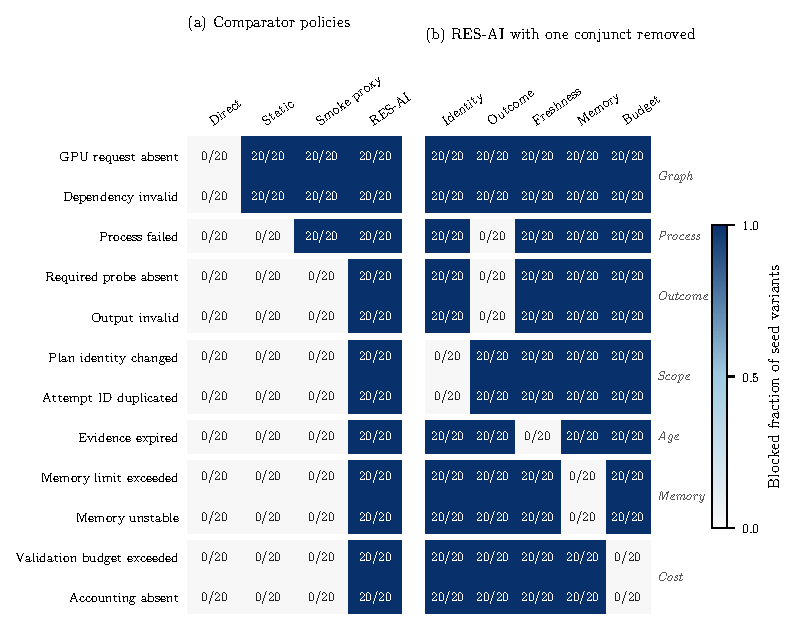
\includegraphics[width=\textwidth]{figures/fault_detection.pdf}
\caption{Blocked variants per fault family, out of \LocalSeeds{} seeds. (a) Comparator policies of the mutation study. (b) Full \tool{} with one conjunct of Equation~\eqref{eq:ready} removed (RQ4). Italic labels group families by the contract concern they violate. Each removed conjunct reopens exactly the families it alone detects.}\label{fig:faults}
\end{figure}

The per-family view (Table~\ref{tab:operators}) explains the aggregate difference. Records with incomplete probe coverage, invalid but present outputs, a changed plan identity, expired evidence, memory violations or invalid accounting all pass both the static validator and the smoke proxy, because each of these faults leaves the job graph valid and the process status successful. A malformed but present output illustrates why file presence is useful for dependencies but insufficient for schema and cardinality. Successful observations of an obsolete plan remain useful history without validating a changed plan.

\paragraph{Threshold sensitivity.} Figure~\ref{fig:sensitivity} shows that every decision boundary moves with its declared parameter and with nothing else. Admission drops from 20/20 to 0/20 between the last grid point at or below $T$ and the first above it (panel a), and between charged totals of 1,200\,s and 1,250\,s when $C=1200$\,s (panel d). For memory headroom (panel b), admission decreases gradually because each seed has its own baseline footprint. At a footprint scale of 1.8, 2, 8 and 9 of 20 seeds remain admissible for $m_{\max}=0.8$, $0.9$ and $0.95$. The static validator and the smoke proxy admit every point of every sweep (dotted lines), because none of the swept properties is visible to them. One implementation detail surfaced at the stability boundary (panel c). When $|m_a-m_b|$ equals $\epsilon$ exactly, 7 of 20 seeds pass for $\epsilon=0.05$ and 15 of 20 for $\epsilon=0.1$, because floating-point rounding of the difference decides the tie. Exact-boundary decisions are therefore not reproducible across inputs, and a production deployment should either quantize telemetry or state a tolerance.

\begin{figure}[t]
\centering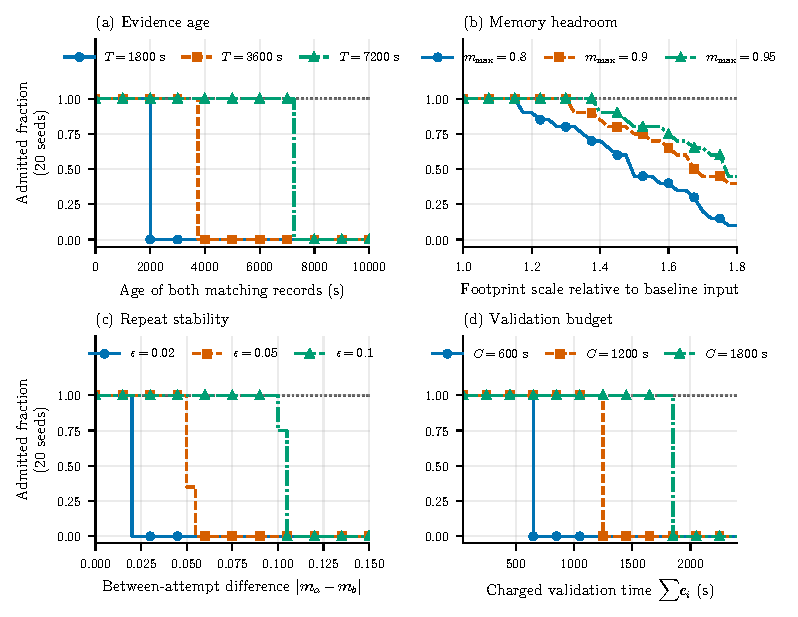
\includegraphics[width=\textwidth]{figures/threshold_sensitivity.pdf}
\caption{Threshold sensitivity of \tool{} admission. Each panel sweeps one evidence property while all other properties remain valid; lines correspond to three settings of the governing parameter and each point aggregates \LocalSeeds{} seeds. The dotted line at 1.0 is shared by the static validator and the smoke proxy, which never respond to these properties. Step lines hold the value until the next grid point.}\label{fig:sensitivity}
\end{figure}

\paragraph{GPU integration.}
% BEGIN inline: generated/gpu_status.tex
All eight CUDA probe records were collected from the two completed GPU array cells (job \code{24888989}), and the dependent analysis job \code{24888990} completed. The clean pair passed the retrospective readiness assessment; corrupted-output, missing-checkpoint and runtime-failure pairs were blocked. Slurm reports 81 allocated MIG-instance seconds across the two cells, with 159 seconds of queue delay for each. The timed probe computations sum to 3.723 instance-seconds; the difference includes environment setup, imports and job overhead. These are measurements of this small integration workload, not saved production compute or evidence about an agent's task accuracy.

% END inline: generated/gpu_status.tex
Table~\ref{tab:gpu} shows that the pilot reproduces two faults that an exit-code check would miss. The corrupt-output processes complete successfully but fail coverage and output validity, and the missing-checkpoint processes produce valid outputs but fail a mandatory obligation. The deliberately raised runtime failure is visible both to status checks and to the readiness rule. Memory headroom is ample in this small workload, so the pilot provides no test of large-model memory pressure.

\begin{table}[t]
\caption{CUDA diagnostics for two repetitions on Nibi. $t_0,t_1$ are timed probe-process seconds. Probes gives the passed obligations out of five in \emph{each} repetition; Output gives valid records out of two. Assessment uses the pair.}\label{tab:gpu}
\small\centering
% BEGIN inline: generated/gpu_diagnostics.tex
\begin{tabularx}{\textwidth}{lrrccY}
\toprule Mode & $t_0$ (s) & $t_1$ (s) & Probes & Output & Assessment / reasons \\
\midrule
Clean & 0.599 & 0.585 & 5/5 & 2/2 & Ready \\
Corrupt output & 0.619 & 0.334 & 4/5 & 0/2 & Blocked: coverage; output validity \\
No checkpoint & 0.458 & 0.440 & 4/5 & 2/2 & Blocked: coverage \\
Runtime failure & 0.366 & 0.322 & 3/5 & 0/2 & Blocked: process failure; coverage; output validity \\
\bottomrule
\end{tabularx}

% END inline: generated/gpu_diagnostics.tex

\end{table}

\begin{tcolorbox}[rqbox, title={Answer to RQ1}]
On constructed faults, evidence-bound admission blocked all \MutationFaultCases{} faulty variants without false blocks, whereas the smoke proxy blocked 25.0\%. Decision boundaries follow the declared parameters exactly, except for floating-point ties at the stability threshold. On real hardware, \tool{} blocked two fault modes that exit statuses did not reveal. These results establish conformance to the specification, not detection rates for natural faults.
\end{tcolorbox}

\subsection{RQ2: Validation cost and its bounds}\label{sec:rq2}
\paragraph{Measured allocation cost.} Figure~\ref{fig:gpu-cost} separates waiting, allocation and probe computation in the Level B pilot. The two GPU cells start after the same 159-second queue delay and consume 39 and 42 allocated MIG-instance seconds. Their timed probe computations sum to 3.723 seconds across all eight records, so timed computation accounts for under 5\% of the allocated cost. Reporting only the inner computation would understate the cost of this integration check roughly twentyfold. The remainder includes setup, imports and execution overhead; the archive does not support a causal decomposition of it.

\begin{figure}[t]
\centering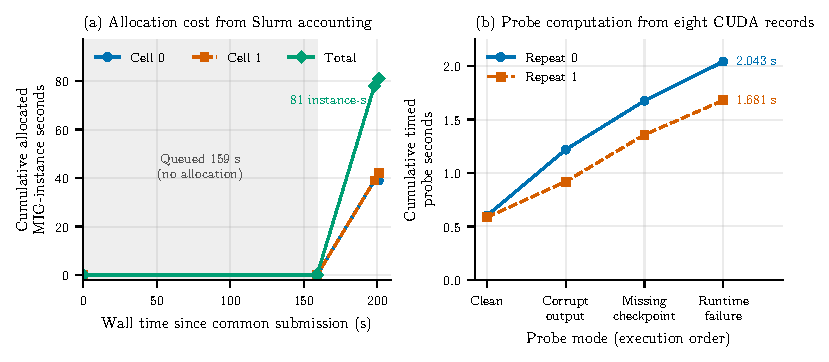
\includegraphics[width=\textwidth]{figures/gpu_cost_timeline.pdf}
\caption{Cost accounting of the Nibi integration pilot. (a) Cumulative allocated MIG-instance seconds reconstructed from Slurm start and end times; queued time accrues no allocated cost. (b) Cumulative timed probe computation in execution order, including the deliberately failing mode. The panels use different accounting boundaries and are not utilization or savings estimates.}\label{fig:gpu-cost}
\end{figure}

\paragraph{Bounded refinement cost.} Figure~\ref{fig:refinement} and Table~\ref{tab:refinement} report the \RefinementEpisodes{} simulated refinement episodes. Charged validation never exceeded the attempt-derived ceiling of $60K$\,s in any episode (Figure~\ref{fig:refinement}b). Mean cost grows with $K$ only until the episodes terminate, then stays flat: additional budget is not consumed once a decision is reached. The cap also limits reachable repairs. With the study setting $K=4$, an initial batch of 64 reached READY in only 2 of 20 episodes, and a batch of 128 in none, because two matching observations plus every failed out-of-memory attempt must fit within $K$. With $K=8$, every initial batch from 16 to 128 converged to READY in the same 14 of 20 episodes, at a mean of 156--336\,s of charged validation. Without declared batch invariance, no proposal was ever produced; episodes that failed with out-of-memory stopped after a single 60-second probe.

\begin{figure}[t]
\centering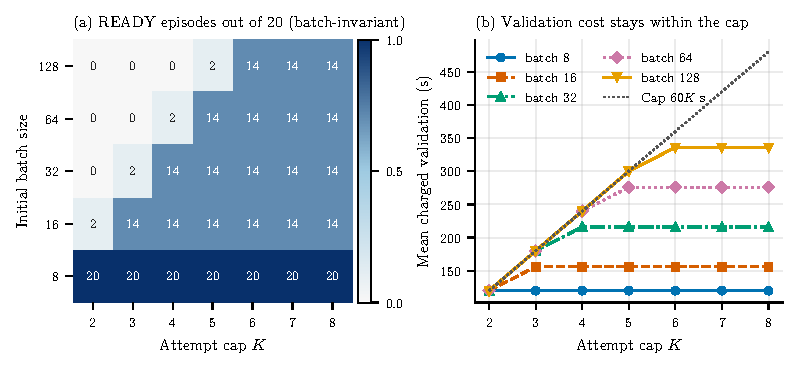
\includegraphics[width=\textwidth]{figures/refinement_bounds.pdf}
\caption{Bounded refinement under the attempt cap $K$ (simulated, batch-invariant contract). (a) Episodes reaching READY out of \LocalSeeds{} seeds by initial batch size and $K$. (b) Mean charged validation time, which never exceeds the $60K$\,s ceiling (dotted) and stops growing once episodes terminate.}\label{fig:refinement}
\end{figure}

\begin{table}[t]
\caption{Terminal decisions of simulated refinement episodes, out of \LocalSeeds{} seeds per row. Ready: READY reached; No prop.: blocked because the contract permitted no further proposal; Cap hit: blocked because the attempt or compute cap was reached; Cost: mean charged validation, with every probe charged 60\,s.}\label{tab:refinement}
\centering\small\setlength{\tabcolsep}{4pt}
% BEGIN inline: generated/refinement_table.tex
\begin{tabular}{lrrrrrrrr}
\toprule & \multicolumn{4}{c}{$K=4$ (study setting)} & \multicolumn{4}{c}{$K=8$} \\
\cmidrule(lr){2-5}\cmidrule(lr){6-9} Initial batch & Ready & \shortstack{No\\prop.} & \shortstack{Cap\\hit} & \shortstack{Cost\\(s)} & Ready & \shortstack{No\\prop.} & \shortstack{Cap\\hit} & \shortstack{Cost\\(s)} \\
\midrule
\multicolumn{9}{l}{\emph{Batch-invariant contract}} \\
\quad 8 & 20 & 0 & 0 & 120 & 20 & 0 & 0 & 120 \\
\quad 16 & 14 & 6 & 0 & 156 & 14 & 6 & 0 & 156 \\
\quad 32 & 14 & 6 & 0 & 216 & 14 & 6 & 0 & 216 \\
\quad 64 & 2 & 0 & 18 & 240 & 14 & 6 & 0 & 276 \\
\quad 128 & 0 & 0 & 20 & 240 & 14 & 6 & 0 & 336 \\
\multicolumn{9}{l}{\emph{Batch invariance not declared}} \\
\quad 8 & 20 & 0 & 0 & 120 & 20 & 0 & 0 & 120 \\
\quad 16 & 2 & 18 & 0 & 84 & 2 & 18 & 0 & 84 \\
\quad 32 & 0 & 20 & 0 & 60 & 0 & 20 & 0 & 60 \\
\quad 64 & 0 & 20 & 0 & 60 & 0 & 20 & 0 & 60 \\
\quad 128 & 0 & 20 & 0 & 60 & 0 & 20 & 0 & 60 \\
\bottomrule
\end{tabular}

% END inline: generated/refinement_table.tex

\end{table}

\paragraph{Assessment overhead.} Figure~\ref{fig:overhead} shows that a readiness assessment costs a median of \OverheadMinMs{}\,ms for a two-record ledger and \OverheadMaxMs{}\,ms for \OverheadMaxAttempts{} records, growing approximately linearly with ledger size. Even at \OverheadMaxAttempts{} records, an assessment costs less than $2\times10^{-4}$ of the shortest measured probe allocation (39\,s). The cost of the gate itself is therefore negligible; the cost of validation lies in the probe allocations it requires.

\begin{figure}[t]
\centering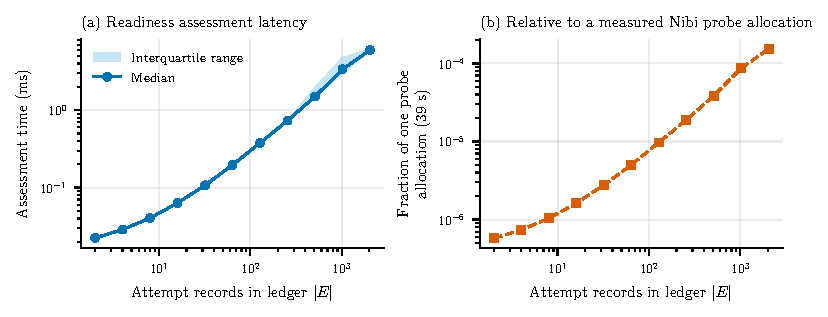
\includegraphics[width=\textwidth]{figures/assessment_overhead.pdf}
\caption{Assessment overhead on the analysis workstation. (a) Median and interquartile range of \OverheadRepeats{} timed calls per ledger size (log--log). (b) The same medians as a fraction of the shortest measured Nibi probe allocation.}\label{fig:overhead}
\end{figure}

\begin{tcolorbox}[rqbox, title={Answer to RQ2}]
Validation cost is dominated by allocations, not by assessment: the pilot's timed computation was under 5\% of its 81 allocated instance-seconds, and the gate costs at most milliseconds. The attempt and compute caps strictly bound charged validation and also limit how many refinements can complete. Whether validation saves resources relative to smoke-then-production remains a campaign question.
\end{tcolorbox}

\subsection{RQ3: Scientific preservation}\label{sec:rq3}
Across the \RefinementEpisodes{} episodes, \tool{} produced \RefinementProposals{} refinement proposals. The hash of the scientific subdocument $S$ was identical before and after each of them (\RefinementScienceChanged{} changes). All proposals came from batch-invariant contracts, and none from contracts without the declaration. This confirms structural preservation: the implementation never rewrites model, data, prompts, seeds or scoring. Structural preservation is necessary but not sufficient for preserving the scientific estimand. Training batch changes can alter optimization, and inference scheduling and numerical nondeterminism can alter outputs.

The deployment case study in Section~\ref{sec:mapcoder-deployment} exercises evidence collection for two model specifications. Semantic preservation under an operational refinement remains untested by executed evidence; the campaign tests it with equivalence margins fixed before comparison.

\begin{tcolorbox}[rqbox, title={Answer to RQ3}]
No refinement proposal altered the scientific specification, and proposals required an explicit batch-invariance declaration. Whether permitted operational changes preserve experimental outcomes, rather than declared fields, has not yet been measured.
\end{tcolorbox}

\subsection{RQ4: Contribution of contract components}\label{sec:rq4}
Table~\ref{tab:ablation} and Figure~\ref{fig:faults}b show that every conjunct is necessary on this suite. Removing any single component reopens exactly the fault families that only it detects, lowering detection to between 75.0\% (Outcome) and 91.7\% (Freshness). No component is redundant: no family is detected by two different components alone, apart from the graph faults that the upstream validator catches under every variant. Removing a component never introduced false blocks. The Outcome component contributes most because it covers three families, but one of those, process failure, is also caught by the smoke proxy. The components that a successful smoke run cannot replace are therefore identity, freshness, memory and budget, together with coverage and output validity.

\begin{table}[t]
\caption{Leave-one-conjunct-out ablation on the mutation suite (\MutationFaultCases{} faulty and \MutationCleanCases{} clean cases per variant). No variant blocked a clean control.}\label{tab:ablation}
\small\setlength{\tabcolsep}{4pt}
% BEGIN inline: generated/ablation_table.tex
\begin{tabularx}{\textwidth}{llrrY}
\toprule Variant & Removed terms of Eq.~(\ref{eq:ready}) & Blocked & Det.\ (\%) & Fault families that escape \\
\midrule
Full \tool{} & none & 240/240 & 100.0 & none \\
$-$Identity & $h_i=h$; distinct IDs &200/240 & 83.3 & Plan identity changed; Attempt ID duplicated \\
$-$Outcome & $\operatorname{OK}$; $O\subseteq C_i$; output &180/240 & 75.0 & Process failed; Required probe absent; Output invalid \\
$-$Freshness & $t-t_i\leq T$ &220/240 & 91.7 & Evidence expired \\
$-$Memory & $m_i\leq m_{\max}$; $\Delta_{\mathrm{smoke}}\leq\epsilon$ &200/240 & 83.3 & Memory limit exceeded; Memory unstable \\
$-$Budget & $|E|\leq K$; $\sum c_i\leq C$; valid $c_i$ &200/240 & 83.3 & Validation budget exceeded; Accounting absent \\
\bottomrule
\end{tabularx}

% END inline: generated/ablation_table.tex

\end{table}

The refinement study exposes a gap that the ablation cannot. In \HeadroomGapSeeds{} of 20 seeds, halving the batch produced a peak footprint between 0.9 and 1.0 of device capacity (Table~\ref{tab:refinement}, column ``No prop.''). This violates $m_{\max}$ but does not fail with out-of-memory. The Memory conjunct correctly blocks these plans. However, the single implemented refinement fires only on an out-of-memory classification, so it proposes nothing, and the episode stops even though one further halving would satisfy the contract. The memory conjunct and the refinement rule thus use different triggers. Aligning them is a direct improvement for future versions.

\begin{tcolorbox}[rqbox, title={Answer to RQ4}]
Each of the five components of Equation~\eqref{eq:ready} detects fault families that no other component and no smoke check detects, so none can be removed without reopening an escape path. The refinement rule is narrower than the memory conjunct and misses headroom violations that do not fail with out-of-memory.
\end{tcolorbox}


\subsection{Research-artifact deployment with two local models}\label{sec:mapcoder-deployment}

% BEGIN inline: generated/mapcoder_status.tex
Two independent executions of each local-model configuration solved HumanEval/0, made eight model calls each, and passed imports, model initialization, task execution, output schema/cardinality, and persisted-result resume. Both collection-time readiness assessments and input/graph-verifying dispatch dry runs passed; neither dry run submitted production work. Table~\ref{tab:mapcoder-models} separates timed process duration from the enclosing H100 allocation. The Qwen3.8 workflow additionally consumed 86 H100 allocation-seconds in a failed identity-check attempt before any inference, giving 634 H100 seconds including recovery. The adapter had equated the stored manifest checksum with Ollama's advertised model digest; the correction pins and checks both identities separately and was validated in a CPU-only preflight before a fresh GPU run. Canceled pending submissions and CPU download, preparation, inspection and collection jobs remain in the accounting archive; they are not added to GPU seconds. The successful Qwen3.8 repeats each generated 3,286 tokens across their eight calls. Its sampled device-memory fraction was 0.2393 in both repeats, whereas the original backend's PyTorch allocator peaks were approximately 0.1817 and 0.1815. These memory measures have different boundaries and are not directly comparable. The model change creates a different scientific specification; it is not a semantics-preserving execution refinement. Four executions of one task establish bounded deployment and evidence collection, not published benchmark accuracy, statistical superiority, or resource savings.

% END inline: generated/mapcoder_status.tex


\begin{table}[t]
\caption{Observed MapCoder deployment results on HumanEval/0. Each row contains two fresh repeated processes on one full H100. Process time includes each adapter's initialization and inference; allocation time includes the enclosing setup and job overhead. The Qwen3.8 allocation column excludes its separately reported failed attempt. These are distinct scientific configurations, not a paired model-performance benchmark.}\label{tab:mapcoder-models}
\small
% BEGIN inline: generated/mapcoder_table.tex
\begin{tabularx}{\textwidth}{Yrrrrl}
\toprule Model & Solved & Calls & Process (s) & Alloc. (s) & Gate \\
\midrule
Qwen2.5-Coder-7B & 2/2 & 16 & 335.276 & 383 & pass \\
Qwen3.8-27B Q4\_K\_M & 2/2 & 16 & 454.072 & 548 & pass \\
\bottomrule
\end{tabularx}

% END inline: generated/mapcoder_table.tex

\end{table}

\subsection{Completed ChatDev comparative subset}\label{sec:chatdev-results}
\paragraph{Qualified outcomes.} Matching collected episode receipts against the resolved subset ledger yields all $7\times5\times4=140$ required cells, excluding the historical quarantined attempts. Table~\ref{tab:chatdev} separates valid clean production, clean blocking, fault blocking and invalid production. Across conditions, there are 34 valid production outcomes, 61 policy-blocked cases and 45 invalid production outcomes. ``Complete'' means that every required case has a qualified resolved outcome, not that every generated program succeeds. The generated table and its episode-level CSV are reproducible with \code{experiments/make\_campaign\_paper\_artifacts.py}.

\begin{table}[t]
\caption{Completed ChatDev subset: five clean and fifteen injected-fault cases per condition. Clean valid means oracle-valid production; fault invalid means a fault reached production and its result was invalid. Counts describe one artifact and five paired task/seed blocks; they are not independent artifact replications.}\label{tab:chatdev}
\centering\small\setlength{\tabcolsep}{3pt}

% BEGIN inline: generated/chatdev_table.tex
\begin{tabular}{lrrrr}
\toprule
Condition & Clean valid & Clean blocked & Fault blocked & Fault invalid \\
\midrule
Direct native & 5 & 0 & 0 & 15 \\
Upstream static & 5 & 0 & 0 & 15 \\
Upstream smoke & 5 & 0 & 10 & 5 \\
Full \tool{} & 5 & 0 & 15 & 0 \\
No coverage & 5 & 0 & 10 & 5 \\
No identity/freshness & 5 & 0 & 10 & 5 \\
No refinement & 4 & 1 & 15 & 0 \\
\bottomrule
\end{tabular}

% END inline: generated/chatdev_table.tex

\end{table}

Full \tool{} blocks all fifteen injected-fault cases and completes all five clean cases. Direct native and upstream static execution block none of the injected faults and produce invalid outcomes for all fifteen. Upstream smoke and no-coverage each block ten faults but admit all five output-contract faults. No-identity/freshness blocks ten faults but admits all five environment-fault cases involving replayed evidence. No-refinement blocks all fifteen faults and completes four clean cases; its remaining clean case is blocked after an HTTP 500 setup failure with zero completed model calls. This observed clean-case block is retained, but cannot be attributed causally to disabling refinement: batch invariance is false and no operational refinement is permitted for this adapter. Likewise, blocking the injected CPU-residency fault establishes detection of that deployment mismatch, not robustness to out-of-memory or distributed failures. These observations extend RQ1 and the descriptive component comparison in RQ4 without testing artifact-level generality or RQ3 output equivalence.

\paragraph{Cost and remaining work.} The latest collected campaign report (28 October 2026) records 24,752 H100 allocation-seconds (6\,h 52\,min 32\,s), with no outstanding reservations, against the initial 86,400-second cap. This is the campaign total, including native feasibility, controls, failed and quarantined attempts and comparative execution; it is not ChatDev's condition-level cost or an estimate of savings. The pilot allocations are archived separately. All 158 collected campaign archive checksums verify. Native validations for ChatDev, AgentCoder and SWE-agent pass; RepairAgent has dependency/import success but no completed native task, and MetaGPT remains blocked by its unavailable pinned \code{lancedb==0.4.0}. The other eleven comparative subsets have not started. Consequently, campaign progress is 140 of 1,680 potential episodes, and the planned cross-artifact failure-penalized cost and equivalence analyses remain pending.

% END inline: sections/results.tex


% BEGIN inline: sections/discussion.tex
\section{Discussion}\label{sec:discussion}
\subsection{Readiness as scoped evidence}
Readiness is useful when expressed as evidence with scope. A researcher can explain eligibility, a reviewer can identify tested deployment conditions, and an adopter can determine what must be repeated on a different cluster. Explicit incompleteness is actionable: missing distributed evidence calls for another probe or a narrower claim rather than unqualified extrapolation from a local run. The ablation supports this framing. Every conjunct detected faults that a successful smoke run did not reveal (Section~\ref{sec:rq4}), so a smoke run's success should be reported with the obligations it exercised and the plan it described.

The executed analyses also show where the specification needs refinement. Ties at the stability threshold depend on floating-point rounding (Section~\ref{sec:rq1}), and the refinement rule reacts to out-of-memory failures but not to headroom violations that stop short of failure (Section~\ref{sec:rq4}). Both are implementation-level gaps, found by exercising the contract systematically rather than by inspecting individual runs. This supports making such analyses part of the artifact rather than a one-off check.

\subsection{Resource efficiency is comparative}
Resource efficiency is a comparative outcome rather than a property conferred by smoke tests. Validation consumes time and can hold scarce devices. For short reliable workloads, direct execution may be cheaper; for long workloads with detectable early faults, bounded validation may help. A simple break-even condition is $C_{\mathrm{validation}}<pC_{\mathrm{avoidable\ failure}}$, where $p$ is the deployment-specific probability of a failure that the probes actually detect. Neither $p$ nor avoided production cost is estimated by the controller studies. The pilot and aggregate campaign accounting measure incurred costs, but the descriptive ChatDev outcomes do not yet estimate the paired failure-penalized resource endpoint or a natural fault probability. Assessment itself is negligible (Section~\ref{sec:rq2}), allocation overhead dominated the pilot's probe computation, and the attempt cap bounds charged validation at $K$ probe allocations. A team's saved allocation also does not establish cluster-wide utilization gains.

The cap is a policy lever with a visible trade-off. A small $K$ bounds cost tightly but prevents refinements that need several halvings from completing (Table~\ref{tab:refinement}); a larger $K$ admits them at proportionally higher validation cost. The choice should follow from the expected cost of a production failure, not from a default.

\subsection{Bounded automation must preserve the research question}
An agent can make a workflow run by changing models, tasks or numerical settings, potentially invalidating the original experiment. The scientific/execution distinction makes that change reviewable, and the refinement study confirms that the implementation never altered $S$. Semantic preservation still needs evidence, and batch invariance is particularly workload-dependent. Our refinement is consequently a constrained proposal, not unrestricted self-repair.

\subsection{Self-application}
An approach for managing HPC experiments itself requires HPC experiments to establish its value. We therefore applied its staged workflow to its own development, progressing from local contract checks to a bounded CUDA integration run then to the two-model MapCoder case study and a completed ChatDev subset of the twelve-artifact campaign. This makes the proposed discipline concrete: preserve failed or canceled submissions, bind evidence to the configuration actually tested, and require review before expanding the experimental scope. The MapCoder submissions illustrate the point. Three requests were retired before execution, after a configuration defect and unavailable capacity were identified, and each resource-plan change invalidated earlier evidence while the scientific configuration remained fixed. Scheduler admission remains an external constraint; a queued request provides no execution evidence. Self-application can expose implementation and operational defects, but it is not independent validation of effectiveness.

\subsection{Transfer}
Generality depends on transfer conditions. The candidate artifacts vary in workflow, but several depend on cloud APIs or containers, requirements that MCP does not resolve. The likely transferable mechanism is the contract and evidence schema; probes, oracles and feasible resource requests remain artifact- and site-specific. Current evidence supports a reproducible prototype and a descriptive completed comparison for ChatDev; eleven remaining comparisons prevent a claim of benefit across twelve diverse studies.

\section{Threats to Validity}\label{sec:threats}
\textbf{Construct validity.} Synthetic mutations measure policy behavior on supplied records, not scientific correctness or actual failures prevented. The smoke proxy approximates selected upstream checks. The refinement simulation assumes memory linear in batch size and a fixed per-probe cost, so its convergence counts describe the control loop under that model, not real workloads. Framework-allocated memory excludes some driver and process overhead; the Ollama variant instead reports device memory sampled every 0.5 s, which can miss transient peaks and includes a different memory boundary. The small CUDA network does not approximate long-context inference, agent coordination or training. Retrospective identities in the integration analysis are not pre-execution certificates.

\textbf{Internal validity.} The same developer designed the policy, the operators, the ablation grouping and the oracle, creating favorable-test risk. The ablation removes reason codes after assessment, which is equivalent to removing a conjunct only because every conjunct is evaluated independently. The assessment returns early for nonnumeric telemetry, which the Budget group absorbs. Malformed records may be rejected or raise errors; the prototype has not undergone exhaustive fuzzing. Operator-controlled records can omit costs or assert false coverage. The wrapper is bypassable and has a verification-to-execution race. Inherited completion markers are not content-addressed and can reuse state in ways not fully protected by the wrapper. These limitations prevent security and end-to-end correctness claims.

\textbf{External validity.} The Nibi pilots and single-artifact ChatDev subset cannot establish cross-site effects, network behavior or fair-share outcomes. Overhead was timed on one workstation, so absolute latencies will differ elsewhere, although the comparison with probe allocations spans four orders of magnitude. The twelve candidates are purposively selected and concentrated in generation and repair. Current repositories may differ from paper versions; ChatDev uses an explicitly recorded legacy selection, and comparison eligibility for the remaining artifacts is still incomplete. API and local-inference workloads have different accounting boundaries. No many-day, multi-node or 64-GPU production experiment is evaluated.

\textbf{Conclusion validity.} Seed variants are not independent studies and receive no inferential tests; deterministic sweeps report exact counts rather than estimates. Only one artifact has a completed comparative subset, and its five task/seed blocks are nested observations. The no-refinement clean block followed an observed setup failure and cannot identify a refinement effect. Three ineffective fault-injection attempts were quarantined and the resource operator amended; these corrections are disclosed rather than treated as confirmatory evidence from an unchanged protocol. The planned campaign has a small effective sample and may not establish equivalence. Selecting after outcomes, excluding failed installations or counting successful jobs alone would bias results; the protocol retains such records. Compute savings, long-run reliability and widespread adoption remain hypotheses.

\textbf{Reproducibility.} The execution templates are pinned and attributed. Numbers from the unpublished support manuscript are not reused as new findings. The archive retains controller decisions, ablation, sensitivity, refinement and overhead records, seeds, source hashes, repository-availability records, pilot evidence, and qualified and quarantined campaign receipts, and every reported number is regenerated from them. Identity does not capture undeclared dependencies. Release licensing and archival metadata require finalization before public distribution.

\section{Conclusion}\label{sec:conclusion}
\tool{} makes readiness an explicit, bounded decision over identity, coverage and observed resource behavior. The prototype adds assessment and constrained refinement proposals above existing Slurm machinery and exposes them through MCP. The executed studies show that the full contract blocks every constructed fault without false blocks, and that each of its five components is necessary. They also show that decisions follow the declared parameters, that charged validation stays within its cap while proposals leave the scientific specification unchanged, and that assessment costs milliseconds. They also exposed two specification gaps: floating-point ties at the stability threshold and a refinement trigger narrower than the memory conjunct. The GPU pilot exercises limited integration on real hardware. A separate one-task MapCoder case study completed two fresh repeats for each of two local-model configurations, including quantized Qwen3.8-27B; all four solved the task and satisfied the declared probes. The recovered identity-check failure remains charged in allocation accounting. The completed ChatDev subset adds 140 qualified comparative episodes: the full policy blocks fifteen injected-fault cases and completes five clean cases, while smoke-then-production blocks ten faults. Historical ineffective injections and their costs remain archived, with three attempts excluded from qualified outcomes. This is descriptive evidence from one artifact, not cross-artifact generality, semantic equivalence or comparative savings. Eleven remaining artifact comparisons and the planned cost/equivalence analyses are needed to assess transfer and resource benefit.

% END inline: sections/discussion.tex


\section*{Declarations}
\textbf{Funding.} Funding and resource acknowledgements require author confirmation before submission.\\
\textbf{Competing interests.} The author develops the prototype and reused execution framework; no independent evaluator is claimed.\\
\textbf{Human participants.} The reported controller and GPU-probe experiments involve no human-subject data.\\
\textbf{Data and code availability.} Code, observations, analysis, the completed ChatDev subset and the remaining campaign protocol accompany the RES-AI repository. Execution templates originate from \url{https://github.com/ai4se4ai-lab/use-hpc}, pinned in \code{hpc/UPSTREAM.json}. A permanent artifact DOI has not been assigned.\\
\textbf{Use of generative AI.} AI coding and writing assistance was used to implement the prototype, draft the manuscript and conduct three methodological, architectural and literature reviews. These reviews do not constitute independent human peer review. The author must verify final claims, citations and journal-specific disclosure before submission.
\bibliography{bibliography}
\end{document}
